% Options for packages loaded elsewhere
\PassOptionsToPackage{unicode}{hyperref}
\PassOptionsToPackage{hyphens}{url}
\PassOptionsToPackage{dvipsnames,svgnames,x11names}{xcolor}
%
\documentclass[
  b5paper,
  DIV=11,
  numbers=noendperiod]{scrreprt}

\usepackage{amsmath,amssymb}
\usepackage{iftex}
\ifPDFTeX
  \usepackage[T1]{fontenc}
  \usepackage[utf8]{inputenc}
  \usepackage{textcomp} % provide euro and other symbols
\else % if luatex or xetex
  \usepackage{unicode-math}
  \defaultfontfeatures{Scale=MatchLowercase}
  \defaultfontfeatures[\rmfamily]{Ligatures=TeX,Scale=1}
\fi
\usepackage{lmodern}
\ifPDFTeX\else  
    % xetex/luatex font selection
\fi
% Use upquote if available, for straight quotes in verbatim environments
\IfFileExists{upquote.sty}{\usepackage{upquote}}{}
\IfFileExists{microtype.sty}{% use microtype if available
  \usepackage[]{microtype}
  \UseMicrotypeSet[protrusion]{basicmath} % disable protrusion for tt fonts
}{}
\makeatletter
\@ifundefined{KOMAClassName}{% if non-KOMA class
  \IfFileExists{parskip.sty}{%
    \usepackage{parskip}
  }{% else
    \setlength{\parindent}{0pt}
    \setlength{\parskip}{6pt plus 2pt minus 1pt}}
}{% if KOMA class
  \KOMAoptions{parskip=half}}
\makeatother
\usepackage{xcolor}
\ifLuaTeX
  \usepackage{luacolor}
  \usepackage[soul]{lua-ul}
\else
  \usepackage{soul}
  
\fi
\setlength{\emergencystretch}{3em} % prevent overfull lines
\setcounter{secnumdepth}{3}
% Make \paragraph and \subparagraph free-standing
\makeatletter
\ifx\paragraph\undefined\else
  \let\oldparagraph\paragraph
  \renewcommand{\paragraph}{
    \@ifstar
      \xxxParagraphStar
      \xxxParagraphNoStar
  }
  \newcommand{\xxxParagraphStar}[1]{\oldparagraph*{#1}\mbox{}}
  \newcommand{\xxxParagraphNoStar}[1]{\oldparagraph{#1}\mbox{}}
\fi
\ifx\subparagraph\undefined\else
  \let\oldsubparagraph\subparagraph
  \renewcommand{\subparagraph}{
    \@ifstar
      \xxxSubParagraphStar
      \xxxSubParagraphNoStar
  }
  \newcommand{\xxxSubParagraphStar}[1]{\oldsubparagraph*{#1}\mbox{}}
  \newcommand{\xxxSubParagraphNoStar}[1]{\oldsubparagraph{#1}\mbox{}}
\fi
\makeatother

\usepackage{color}
\usepackage{fancyvrb}
\newcommand{\VerbBar}{|}
\newcommand{\VERB}{\Verb[commandchars=\\\{\}]}
\DefineVerbatimEnvironment{Highlighting}{Verbatim}{commandchars=\\\{\}}
% Add ',fontsize=\small' for more characters per line
\usepackage{framed}
\definecolor{shadecolor}{RGB}{241,243,245}
\newenvironment{Shaded}{\begin{snugshade}}{\end{snugshade}}
\newcommand{\AlertTok}[1]{\textcolor[rgb]{0.68,0.00,0.00}{#1}}
\newcommand{\AnnotationTok}[1]{\textcolor[rgb]{0.37,0.37,0.37}{#1}}
\newcommand{\AttributeTok}[1]{\textcolor[rgb]{0.40,0.45,0.13}{#1}}
\newcommand{\BaseNTok}[1]{\textcolor[rgb]{0.68,0.00,0.00}{#1}}
\newcommand{\BuiltInTok}[1]{\textcolor[rgb]{0.00,0.23,0.31}{#1}}
\newcommand{\CharTok}[1]{\textcolor[rgb]{0.13,0.47,0.30}{#1}}
\newcommand{\CommentTok}[1]{\textcolor[rgb]{0.37,0.37,0.37}{#1}}
\newcommand{\CommentVarTok}[1]{\textcolor[rgb]{0.37,0.37,0.37}{\textit{#1}}}
\newcommand{\ConstantTok}[1]{\textcolor[rgb]{0.56,0.35,0.01}{#1}}
\newcommand{\ControlFlowTok}[1]{\textcolor[rgb]{0.00,0.23,0.31}{\textbf{#1}}}
\newcommand{\DataTypeTok}[1]{\textcolor[rgb]{0.68,0.00,0.00}{#1}}
\newcommand{\DecValTok}[1]{\textcolor[rgb]{0.68,0.00,0.00}{#1}}
\newcommand{\DocumentationTok}[1]{\textcolor[rgb]{0.37,0.37,0.37}{\textit{#1}}}
\newcommand{\ErrorTok}[1]{\textcolor[rgb]{0.68,0.00,0.00}{#1}}
\newcommand{\ExtensionTok}[1]{\textcolor[rgb]{0.00,0.23,0.31}{#1}}
\newcommand{\FloatTok}[1]{\textcolor[rgb]{0.68,0.00,0.00}{#1}}
\newcommand{\FunctionTok}[1]{\textcolor[rgb]{0.28,0.35,0.67}{#1}}
\newcommand{\ImportTok}[1]{\textcolor[rgb]{0.00,0.46,0.62}{#1}}
\newcommand{\InformationTok}[1]{\textcolor[rgb]{0.37,0.37,0.37}{#1}}
\newcommand{\KeywordTok}[1]{\textcolor[rgb]{0.00,0.23,0.31}{\textbf{#1}}}
\newcommand{\NormalTok}[1]{\textcolor[rgb]{0.00,0.23,0.31}{#1}}
\newcommand{\OperatorTok}[1]{\textcolor[rgb]{0.37,0.37,0.37}{#1}}
\newcommand{\OtherTok}[1]{\textcolor[rgb]{0.00,0.23,0.31}{#1}}
\newcommand{\PreprocessorTok}[1]{\textcolor[rgb]{0.68,0.00,0.00}{#1}}
\newcommand{\RegionMarkerTok}[1]{\textcolor[rgb]{0.00,0.23,0.31}{#1}}
\newcommand{\SpecialCharTok}[1]{\textcolor[rgb]{0.37,0.37,0.37}{#1}}
\newcommand{\SpecialStringTok}[1]{\textcolor[rgb]{0.13,0.47,0.30}{#1}}
\newcommand{\StringTok}[1]{\textcolor[rgb]{0.13,0.47,0.30}{#1}}
\newcommand{\VariableTok}[1]{\textcolor[rgb]{0.07,0.07,0.07}{#1}}
\newcommand{\VerbatimStringTok}[1]{\textcolor[rgb]{0.13,0.47,0.30}{#1}}
\newcommand{\WarningTok}[1]{\textcolor[rgb]{0.37,0.37,0.37}{\textit{#1}}}

\providecommand{\tightlist}{%
  \setlength{\itemsep}{0pt}\setlength{\parskip}{0pt}}\usepackage{longtable,booktabs,array}
\usepackage{calc} % for calculating minipage widths
% Correct order of tables after \paragraph or \subparagraph
\usepackage{etoolbox}
\makeatletter
\patchcmd\longtable{\par}{\if@noskipsec\mbox{}\fi\par}{}{}
\makeatother
% Allow footnotes in longtable head/foot
\IfFileExists{footnotehyper.sty}{\usepackage{footnotehyper}}{\usepackage{footnote}}
\makesavenoteenv{longtable}
\usepackage{graphicx}
\makeatletter
\def\maxwidth{\ifdim\Gin@nat@width>\linewidth\linewidth\else\Gin@nat@width\fi}
\def\maxheight{\ifdim\Gin@nat@height>\textheight\textheight\else\Gin@nat@height\fi}
\makeatother
% Scale images if necessary, so that they will not overflow the page
% margins by default, and it is still possible to overwrite the defaults
% using explicit options in \includegraphics[width, height, ...]{}
\setkeys{Gin}{width=\maxwidth,height=\maxheight,keepaspectratio}
% Set default figure placement to htbp
\makeatletter
\def\fps@figure{htbp}
\makeatother

\usepackage{libertine}
\addtokomafont{disposition}{\rmfamily}
\renewcommand{\ttdefault}{clmt}
\providecommand{\ped}[1]{_\textrm{#1}}
\providecommand{\ap}[1]{^\textrm{#1}}
\providecommand{\app}[1]{^\textrm{#1}}

\providecommand*{\angs}{\smash{\mathrm{\ring A}}}
\providecommand*{\celsius}{\mathrm{~\circ C}}
\providecommand*{\micro}{\mu}

\providecommand*{\unit}[1]{\textrm{\,#1}}


\providecommand{\E}{\mathrm{e}}
\providecommand{\I}{\mathrm{i}}
\providecommand{\sfrac}[2]{^{#1}/_{#2}}

\providecommand{\conc}[1]{\left[\mathrm{#1}\right]}


\providecommand{\command}[1]{\textsl{#1}}
\providecommand{\out}[1]{\begin{verbatim}#1\end{verbatim}}


\providecommand{\diff}{\mathrm{d}\,}


\providecommand*{\deriv}[3][]{% arguments: order of the derivative(optional), function, variable
	\frac{\diff^{#1}#2}{\diff #3^{#1}}}
\providecommand*{\pderiv}[3][]{% arguments: order of the derivative(optional), function, variable
	\frac{\partial^{#1}#2}
		{\partial #3^{#1}}}
  
\renewcommand{\vec}[1]{{\boldsymbol #1}}

\providecommand{\cov}[2]{\mathrm{Cov}\!\left(#1, #2\right)}
\providecommand{\var}[1]{\mathrm{Var}\!\left(#1\right)}

\providecommand{\mean}[1]{\overline{#1}}

\providecommand{\sd}[1]{\sigma\left(#1\right)}
\providecommand{\ev}[1]{\mathbb{E}\!\left(#1\right)}
\providecommand{\pr}[1]{\textrm{Pr}\!\left(#1\right)}

\KOMAoption{captions}{tableheading}
\makeatletter
\@ifpackageloaded{tcolorbox}{}{\usepackage[skins,breakable]{tcolorbox}}
\@ifpackageloaded{fontawesome5}{}{\usepackage{fontawesome5}}
\definecolor{quarto-callout-color}{HTML}{909090}
\definecolor{quarto-callout-note-color}{HTML}{0758E5}
\definecolor{quarto-callout-important-color}{HTML}{CC1914}
\definecolor{quarto-callout-warning-color}{HTML}{EB9113}
\definecolor{quarto-callout-tip-color}{HTML}{00A047}
\definecolor{quarto-callout-caution-color}{HTML}{FC5300}
\definecolor{quarto-callout-color-frame}{HTML}{acacac}
\definecolor{quarto-callout-note-color-frame}{HTML}{4582ec}
\definecolor{quarto-callout-important-color-frame}{HTML}{d9534f}
\definecolor{quarto-callout-warning-color-frame}{HTML}{f0ad4e}
\definecolor{quarto-callout-tip-color-frame}{HTML}{02b875}
\definecolor{quarto-callout-caution-color-frame}{HTML}{fd7e14}
\makeatother
\makeatletter
\@ifpackageloaded{bookmark}{}{\usepackage{bookmark}}
\makeatother
\makeatletter
\@ifpackageloaded{caption}{}{\usepackage{caption}}
\AtBeginDocument{%
\ifdefined\contentsname
  \renewcommand*\contentsname{Inhoudsopgave}
\else
  \newcommand\contentsname{Inhoudsopgave}
\fi
\ifdefined\listfigurename
  \renewcommand*\listfigurename{Lijst van figuren}
\else
  \newcommand\listfigurename{Lijst van figuren}
\fi
\ifdefined\listtablename
  \renewcommand*\listtablename{Lijst van tabellen}
\else
  \newcommand\listtablename{Lijst van tabellen}
\fi
\ifdefined\figurename
  \renewcommand*\figurename{Figuur}
\else
  \newcommand\figurename{Figuur}
\fi
\ifdefined\tablename
  \renewcommand*\tablename{Tabel}
\else
  \newcommand\tablename{Tabel}
\fi
}
\@ifpackageloaded{float}{}{\usepackage{float}}
\floatstyle{ruled}
\@ifundefined{c@chapter}{\newfloat{codelisting}{h}{lop}}{\newfloat{codelisting}{h}{lop}[chapter]}
\floatname{codelisting}{Listing}
\newcommand*\listoflistings{\listof{codelisting}{Lijst van listings}}
\usepackage{amsthm}
\theoremstyle{definition}
\newtheorem{exercise}{Oefening}[chapter]
\theoremstyle{remark}
\AtBeginDocument{\renewcommand*{\proofname}{Bewijs}}
\newtheorem*{remark}{Opmerking}
\newtheorem*{solution}{Oplossing}
\newtheorem{refremark}{Opmerking}[chapter]
\newtheorem{refsolution}{Oplossing}[chapter]
\makeatother
\makeatletter
\makeatother
\makeatletter
\@ifpackageloaded{caption}{}{\usepackage{caption}}
\@ifpackageloaded{subcaption}{}{\usepackage{subcaption}}
\makeatother
\newcounter{quartocallouttipno}
\newcommand{\quartocallouttip}[1]{\refstepcounter{quartocallouttipno}\label{#1}}

\ifLuaTeX
\usepackage[bidi=basic]{babel}
\else
\usepackage[bidi=default]{babel}
\fi
\babelprovide[main,import]{dutch}
% get rid of language-specific shorthands (see #6817):
\let\LanguageShortHands\languageshorthands
\def\languageshorthands#1{}
\ifLuaTeX
  \usepackage{selnolig}  % disable illegal ligatures
\fi
\usepackage{bookmark}

\IfFileExists{xurl.sty}{\usepackage{xurl}}{} % add URL line breaks if available
\urlstyle{same} % disable monospaced font for URLs
\hypersetup{
  pdftitle={Kwantitatieve Biologie},
  pdfauthor={Vakgroep Biologie, Universiteit Utrecht},
  pdflang={nl},
  colorlinks=true,
  linkcolor={blue},
  filecolor={Maroon},
  citecolor={Blue},
  urlcolor={Blue},
  pdfcreator={LaTeX via pandoc}}


\title{Kwantitatieve Biologie}
\author{Vakgroep Biologie, Universiteit Utrecht}
\date{2024-06-20}

\begin{document}
\maketitle

\renewcommand*\contentsname{Inhoudsopgave}
{
\hypersetup{linkcolor=}
\setcounter{tocdepth}{2}
\tableofcontents
}

\part{Kwantitatieve Biologie}

\part{Introductie tot programmeren}

Biologie in de 21e eeuw vereist analyse van grote hoeveelheden data, en
modellering om complexe biologische systemen beter te begrijpen en te
voorspellen. In dit onderdeel van de cursus maak je kort kennis met de
basisprincipes van R, zodat ook jij straks voorspellingen kan doen, kan
aantonen of een gemeten verschil statistisch significant is, en mooie
grafieken kan maken.

\includegraphics[width=7.29167in,height=\textheight]{Programmeren/figuren/rfrogs.png}
Om kikkers te begrijpen kunnen we niet alleen heel hard naar kikkers
kijken (afbeelding gegenereerd met Dall-E, juli 2024)

\chapter{Dag 1: beginnen met Rstudio}\label{dag-1-beginnen-met-rstudio}

\ul{Stap 1: R zelf installeren.}

R kun je eenvoudig installeren via de
\href{https://cran.r-project.org/}{CRAN website}.

\begin{itemize}
\item
  Windows-gebruikers: ga naar ``Download R for Windows'', klikken op de
  link ``base'' en vervolgens op de link ``Download R x.x.x for
  Windows'' om het installatiebestand te downloaden. Open het
  gedownloade .exe bestand en volg de instructies om R te installeren.
\item
  Mac-gebruikers: ``Download R for (Mac) OS X''. Download het juiste
  installatiebestand voor jouw macOS-versie. Let op: als je een oudere
  Mac gebruikt moet je de ``Intel Mac'' versie downloaden. Open het .pkg
  bestand en volg de instructies.
\end{itemize}

\ul{Stap 2: Rstudio installeren.}

Nadat je R geïnstalleerd hebt, kun je beginnen met het installeren van
Rstudio. Deze downloaden we vanaf de
\href{https://posit.co/download/rstudio-desktop/}{website van Rstudio}.
Deze website legt ook uit dat je wel eerst R moet installeren, maar dat
hebben we al gedaan. We kunnen dus meteen naar stap 2: Install Rstudio.
Deze website herkent vanzelf wel besturingssysteem je gebruikt, dus hoef
je het alleen nog maar te installeren:

\begin{itemize}
\item
  Windows-gebruikers: volg de instructies van de installatie-wizard
\item
  Mac-gebruiker: open de .dmg en sleep `Rstudio' naar je Applications
  folder
\end{itemize}

Nu kun je Rstudio opstarten, en zou alles moeten werken\footnote{In een
  enkel geval kan Rstudio de installatie van R niet automatisch vinden.
  Ga dan naar `Tools' \textgreater{} `Global options', en dan naar het
  tabblad `General'. Hier kan je handmatig instellen waar R
  geïnstalleerd staat. Vraag waar nodig hulp van je student-assistent
  (of ChatGPT ;{]})}

\section{Je eerste script}\label{je-eerste-script}

Nu je Rstudio hebt opgestart, gaan we eerst een nieuw script aanmaken.
Klik hiervoor op de knop \texttt{New\ file} en kies \texttt{R\ script}.
Nu opent zich een nieuw venster, met daar in een \texttt{script} zonder
naam. Sla dit script op op een logische plek. Maar wat is een script
eigenlijk?

Een script is vergelijkbaar met een recept: het bevat de instructies om
iets lekkers te koken, maar niet de ingredienten of het resultaat zelf.
Deze instructies staan in zogeheten ``plain text'' formaat. Dit betekent
dat de tekst geen vetgedrukte woorden, cursief, onderstrepingen, kleuren
of speciale lettertypes bevat. Plain tekst kan data beschrijven
(bijvoorbeeld met elke regel een observatie), of in het geval van een
R-script een set van instructies. Elke regel bevat hoogstens 1
instructie, en deze code kan regel-per-regel worden uitgevoerd, of in
één keer.

Kopieer voor het volgende onderdeel de volgende code naar je eigen
script:

\begin{Shaded}
\begin{Highlighting}[]
\DecValTok{1}\SpecialCharTok{+}\DecValTok{2}
\DecValTok{1}\SpecialCharTok{+}\DecValTok{2{-}3}
\DecValTok{1}\SpecialCharTok{+}\DecValTok{2{-}3}\SpecialCharTok{*}\DecValTok{4}\SpecialCharTok{/}\DecValTok{5}
\end{Highlighting}
\end{Shaded}

\section{Script en console}\label{script-en-console}

In Rstudio kun je op meerdere manieren regels code uitvoeren. Om de code
uit je script regel-per-regel uit te voeren, klik je de bovenste regel
aan (niet selecteren, maar gewoon ergens in de regel klikken), en
gebruik je \texttt{Run\ \textgreater{}\ Run\ Selected\ Line(s)} (de
sneltoets hiervoor is \texttt{Ctrl/Cmd+Enter}, wat heel handig is om in
je vingers te krijgen!). Nu je de eerste regel hebt uitgevoerd, zie je
in de console (onder het script) het antwoord: \texttt{{[}1{]}\ 3}. De
\texttt{{[}1{]}} geeft aan dat dit het eerste (enige) waarde is die de
berekening heeft gegeven. Later zul je zien dat een berekening ook
meerdere waarden terug kan geven. Je kan ook het hele script in één keer
uitvoeren door \texttt{Run\ \textgreater{}\ Run\ all} te kiezen.

De bovenstaande uitleg geeft aan hoe je het script (het ``recept'') uit
kan voeren, maar wat nu als je even snel iets wil uitproberen voordat je
het recept helemaal overhoop gooit? Hiervoor kun je direct in de console
typen. Als je bijvoorbeeld de berekening \texttt{80/250} in de console
typt, heb je gauw een antwoord op je vraag maar is je script niet
aangepast. De console is dus handig om even wat uit te proberen, maar
let op: deze code wordt niet opgeslagen als je het script opslaat!

\section{Rekenen met R}\label{rekenen-met-r}

Zoals je nu misschien begrijpt, is R een geweldig krachtige
rekenmachine! In plaats van alles handmatig uit te rekenen of in je
grafische rekenmachine in te typen, kunnen we onze eigen R-scripts maken
die berekeningen gemakkelijk en reproduceerbaar maken. Om dit nog
makkelijker te maken, kunnen we gebruik maken van variabelen:

\begin{Shaded}
\begin{Highlighting}[]
\CommentTok{\# a, b, en c waardes toekennen (assigning variables)}
\NormalTok{a }\OtherTok{\textless{}{-}} \DecValTok{1}
\NormalTok{b }\OtherTok{\textless{}{-}} \DecValTok{3}
\NormalTok{c }\OtherTok{\textless{}{-}} \FloatTok{2.5}

\CommentTok{\# rekenen met a, b, en c}
\NormalTok{a}\SpecialCharTok{+}\NormalTok{b}\SpecialCharTok{{-}}\NormalTok{c }\CommentTok{\# a plus b min c}
\NormalTok{a}\SpecialCharTok{*}\NormalTok{b  }\CommentTok{\# a maal b}
\NormalTok{a}\SpecialCharTok{/}\NormalTok{b  }\CommentTok{\# a gedeeld door b}
\NormalTok{b}\SpecialCharTok{*}\NormalTok{b  }\CommentTok{\# b maal b}
\NormalTok{b}\SpecialCharTok{\^{}}\DecValTok{2}  \CommentTok{\# b kwadraad}
\FunctionTok{sqrt}\NormalTok{(b) }\CommentTok{\# wortel (sqaure root) van b}


\CommentTok{\# andere manieren om variabelen te definieren}
\DecValTok{3} \OtherTok{{-}\textgreater{}}\NormalTok{ d}
\NormalTok{e }\OtherTok{=} \FloatTok{2.5}

\CommentTok{\# een uitgebreider sommetje uitrekenen}
\NormalTok{d}\SpecialCharTok{/}\NormalTok{e}\SpecialCharTok{+}\NormalTok{d}\SpecialCharTok{*}\NormalTok{(c}\SpecialCharTok{+}\NormalTok{d)}

\CommentTok{\# deze som kunnen we ook weer opslaan in een variabele}
\NormalTok{uitkomst }\OtherTok{\textless{}{-}}\NormalTok{ d}\SpecialCharTok{/}\NormalTok{e}\SpecialCharTok{+}\NormalTok{d}\SpecialCharTok{*}\NormalTok{(c}\SpecialCharTok{+}\NormalTok{d)}
\end{Highlighting}
\end{Shaded}

\section{Comments}\label{sec-environment}

In de bovenstaande code zie je meerdere regels met een hekje (\#)
ervoor. Alle tekst na een hekje wordt door R genegeerd, zodat we onze
code opmerkingen kunnen plaatsen. Deze opmerkingen heten in het Engels
\emph{comments}.

\section{De ``Environment''}\label{de-environment}

Variabelen die je definieert worden opgeslagen in de
\textbf{Environment}. Waar het script een soort ``recept'' is, is de
\textbf{Environment} meer vergelijkbaar met de keukentafel: hier worden
alle ingeladen gegevens, berekeningen, en grafieken opgeslagen terwijl
je aan je gerecht werkt. De environment helpt je om een overzicht te
houden van wat er allemaal gebeurt, en blijft behouden totdat je Rstudio
afsluit. Let op: ook de stapjes die je met de console hebt gedaan komen
op deze keukentafel terecht, maar als je wil dat iemand anders het
gerecht kan maken moet je zorgen dat ook het recept klopt. Dit recept
(het script) is namelijk vaak het enige wat we zullen opslaan. Zo kunnen
we de volgende keer ons gerecht opnieuw maken, of ons gerecht met andere
delen. En let op: als je de volgende keer Rstudio opstart, begin je
opnieuw met koken, en begint je keukentafel dus weer leeg!

\section{Opgave onderdeel 1}\label{opgave-onderdeel-1}

Om te testen of je de informatie uit onderdeel 1 hebt begrepen staat
hier een simpele opgave. Lees de code hierboven nog eens door, en
beantwoord de volgende vragen:

\begin{enumerate}
\def\labelenumi{\arabic{enumi}.}
\tightlist
\item
  Definieer a=2, en reken met R uit wat \(a^3\) is.
\item
  Definieer b=9.5 en reken uit wat \(b^{19}\) is (let op: dit hoeft geen
  lange regel te zijn)
\item
  Stel je zet eerst 3 stappen naar links, dan 4 stappen naar boven, en
  loopt vervolgens terug naar je beginpositie. Schrijf een script met R
  die uitrekent hoe ver je in totaal hebt gelopen. Zorg dat de uitkomst
  van je berekening \textbf{niet} in de environment staat, maar slechts
  in de console wordt weergegeven.
\item
  Bereken nu uit hoever je gelopen zou zijn als je in plaats hiervan 5
  stappen naar links en 6 stappen naar boven had gezet. Zorg dit keer
  dat de uitkomst \textbf{wel} in de environment staat on de de naam
  ``afstand''.
\item
  Voeg de volgende regel toe aan je script:\\
  \texttt{print(paste(\textquotesingle{}Je\ hebt\textquotesingle{},\ afstand,\ \textquotesingle{}stappen\ gelopen\textquotesingle{}))}.
  Voer je hele script uit.
\item
  Sla je script op!
\end{enumerate}

\begin{Shaded}
\begin{Highlighting}[]
\CommentTok{\# Dit is simpelweg de stelling van pythagoras:}
\NormalTok{a }\OtherTok{\textless{}{-}} \DecValTok{5}
\NormalTok{b }\OtherTok{\textless{}{-}} \DecValTok{6}
\NormalTok{c }\OtherTok{\textless{}{-}} \FunctionTok{sqrt}\NormalTok{(a}\SpecialCharTok{\^{}}\DecValTok{2}\SpecialCharTok{+}\NormalTok{b}\SpecialCharTok{\^{}}\DecValTok{2}\NormalTok{)}
\NormalTok{afstand }\OtherTok{\textless{}{-}}\NormalTok{a}\SpecialCharTok{+}\NormalTok{b}\SpecialCharTok{+}\NormalTok{c}
\FunctionTok{print}\NormalTok{(}\FunctionTok{paste}\NormalTok{(}\StringTok{\textquotesingle{}Je hebt\textquotesingle{}}\NormalTok{, afstand, }\StringTok{\textquotesingle{}stappen gelopen\textquotesingle{}}\NormalTok{))}
\end{Highlighting}
\end{Shaded}

\chapter{Dag 2: programmeren met R}\label{dag-2-programmeren-met-r}

\section{Typen variabelen}\label{typen-variabelen}

We hebben in het eerste onderdeel al een beetje kennis gemaakt met
variabelen. Maar je kan in variabelen niet alleen nummers opslaan, maar
ook een heleboel andere type gegevens. De meest belangrijke variabelen
zijn:

\begin{itemize}
\item
  \emph{Numerics} (\texttt{1}, \texttt{2}, \texttt{3}, maar ook
  \texttt{2.158196} zijn \emph{numeric})
\item
  \emph{Logicals} (\texttt{TRUE} en \texttt{FALSE})
\item
  \emph{Strings} (\texttt{"a"}, \texttt{"Hoi"}, of
  \texttt{"bananen\ zijn\ krom"})
\end{itemize}

\section{Geen appels en peren
vergelijken}\label{geen-appels-en-peren-vergelijken}

In R kun je berekeningen uitvoeren, maar je kan natuurlijk geen appels
en peren vergelijken. Bekijk bijvoorbeeld devolgende code:

\begin{Shaded}
\begin{Highlighting}[]
\NormalTok{appels }\OtherTok{\textless{}{-}} \DecValTok{3}
\NormalTok{peren }\OtherTok{\textless{}{-}} \StringTok{"groen"}
\NormalTok{appels }\SpecialCharTok{+}\NormalTok{ peren}
\end{Highlighting}
\end{Shaded}

Als je de bovenstaande code probeert uit te voeren, geeft R een
foutmelding:
\texttt{Error\ in\ appels\ +\ peren\ :\ non-numeric\ argument\ to\ binary\ operator}.
Dat is maar goed ook, want hoewel dit een overduidelijk onzinnige som
is, kan het ook zijn dat je met de beste intenties een foutje maakt!

\section{Data structuren}\label{data-structuren}

Het is vaak heel handig om je variabelen in lijsten of tabellen op te
slaan. Dergelijke lijsten of tabellen worden meestal \emph{data
structures} genoemd. De meest belangrijke data structures in R zijn:

\begin{itemize}
\item
  \emph{Vectors} (lijst van elementen van hetzelfde type)
\item
  \emph{Macrices} (tabel van elementen van hetzelfde type)
\item
  \emph{Dataframes} (tabel waarin elke kolom een ander type data kan
  zijn)
\end{itemize}

\begin{figure}[H]

{\centering 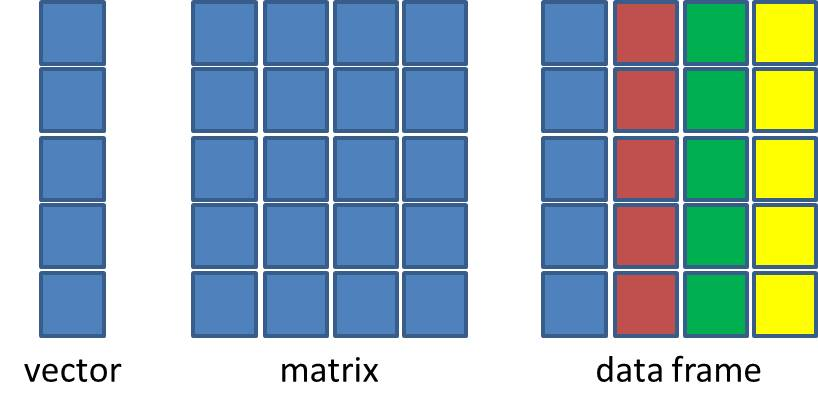
\includegraphics[width=4.16667in,height=\textheight]{Programmeren/figuren/data_structure.jpg}

}

\caption{datastructs}

\end{figure}%

\emph{(figuur is niet van mij, misschien even namaken)}

\subsection{Vectoren}\label{sec-vectoren}

Om een vector te maken, kunnen we deze handmatig intypen:

\begin{Shaded}
\begin{Highlighting}[]
\NormalTok{mijnvector }\OtherTok{\textless{}{-}} \FunctionTok{c}\NormalTok{(}\DecValTok{1}\NormalTok{,}\DecValTok{2}\NormalTok{,}\FloatTok{0.1}\NormalTok{,}\SpecialCharTok{{-}}\DecValTok{5}\NormalTok{)}
\end{Highlighting}
\end{Shaded}

Maar handmatig getallen invoeren is niet altijd handig. Gelukkig kun je
met R een boel lijstjes maken op een snellere manier:

\begin{Shaded}
\begin{Highlighting}[]
\DecValTok{1}\SpecialCharTok{:}\DecValTok{4}                \CommentTok{\# 1, 2, 3, 4}
\DecValTok{5}\SpecialCharTok{:}\DecValTok{2}                \CommentTok{\# 5, 4, 3, 2}
\FunctionTok{rep}\NormalTok{(}\DecValTok{2}\NormalTok{,}\DecValTok{4}\NormalTok{)           }\CommentTok{\# 2, 2, 2, 2}
\FunctionTok{seq}\NormalTok{(}\DecValTok{0}\NormalTok{,}\FloatTok{4.5}\NormalTok{,}\FloatTok{1.5}\NormalTok{)     }\CommentTok{\# 0.0, 1.5, 3.0, 4.5}
\FunctionTok{sample}\NormalTok{(}\DecValTok{1}\SpecialCharTok{:}\DecValTok{6}\NormalTok{,}\DecValTok{4}\NormalTok{)      }\CommentTok{\# 4, 6, 3, 5 (iedere keer anders!)}
\FunctionTok{sample}\NormalTok{(letters,}\DecValTok{4}\NormalTok{)  }\CommentTok{\# "f", "j", "o", "y" (iedere keer anders!)}
\FunctionTok{runif}\NormalTok{(}\DecValTok{2}\NormalTok{)           }\CommentTok{\# 0.9965360 0.8978062 (iedere keer anders!)}
\end{Highlighting}
\end{Shaded}

De laatste vijf regels van het bovenstaande script zijn voorbeelden van
``functies''. Een functie is een herhaalbaar blokje code die je aanroept
met de naam (rep, seq, sample), gevolgd door haakjes met daartussen
eventuele \emph{argumenten}. De functie zet deze argumenten om in een
zogeheete return-waarde, wat bijvoorbeeld een getal of een lijst
getallen is. Je leert meer over functies in het onderdeel
Paragraaf~\ref{sec-functies}.

Je kan met vectoren ook rekenen. Zo kan je bijvoorbeeld twee vectoren
bij elkaar optellen, of één en hetzelfde getal bij alle elementen van
een vector optellen:

\begin{Shaded}
\begin{Highlighting}[]
\CommentTok{\# Rekenen met vectoren}
\NormalTok{x }\OtherTok{\textless{}{-}} \DecValTok{1}\SpecialCharTok{:}\DecValTok{3}           \CommentTok{\# 1, 2, 3}
\NormalTok{x }\SpecialCharTok{+} \DecValTok{10}             \CommentTok{\# 11 12 13}
\NormalTok{y }\OtherTok{\textless{}{-}} \FunctionTok{c}\NormalTok{(}\DecValTok{1}\NormalTok{, }\DecValTok{10}\NormalTok{, }\DecValTok{4}\NormalTok{)   }\CommentTok{\# 1 10 4}
\NormalTok{x }\SpecialCharTok{+}\NormalTok{ y              }\CommentTok{\# 2 12  7}
\NormalTok{x }\SpecialCharTok{*}\NormalTok{ y              }\CommentTok{\# 1 20 12}
\NormalTok{x }\SpecialCharTok{+}\NormalTok{ y }\SpecialCharTok{/} \DecValTok{100}        \CommentTok{\# 1.01 2.10 3.04}
\NormalTok{(x }\SpecialCharTok{+}\NormalTok{ y) }\SpecialCharTok{/} \DecValTok{100}      \CommentTok{\# 0.02 0.12 0.07}
\end{Highlighting}
\end{Shaded}

In de bovenstaande code zie je een subtiel verschil tussen de laatste
twee regels. Net als bij wiskunde gaan delen en vermedigvuldigen altijd
voor, dus moet je soms aangeven in welke volgorde je de berekeninng wil
uitvoeren!

\subsection{Matrices}\label{matrices}

Matrices in R kun je maken door de functie \texttt{matrix} aan te
roepen, die je waarden van de matrix en het aantal rijen als argumenten
geeft:

\begin{Shaded}
\begin{Highlighting}[]
\FunctionTok{matrix}\NormalTok{(}\FunctionTok{c}\NormalTok{(}\DecValTok{1}\NormalTok{, }\DecValTok{2}\NormalTok{, }\DecValTok{3}\NormalTok{, }\DecValTok{4}\NormalTok{,}\DecValTok{5}\NormalTok{, }\DecValTok{6}\NormalTok{, }\DecValTok{7}\NormalTok{, }\DecValTok{8}\NormalTok{, }\DecValTok{9}\NormalTok{), }\AttributeTok{nrow=}\DecValTok{3}\NormalTok{)}
\FunctionTok{matrix}\NormalTok{(}\FunctionTok{c}\NormalTok{(}\DecValTok{1}\NormalTok{, }\DecValTok{2}\NormalTok{, }\DecValTok{3}\NormalTok{, }\DecValTok{4}\NormalTok{,}\DecValTok{5}\NormalTok{, }\DecValTok{6}\NormalTok{, }\DecValTok{7}\NormalTok{, }\DecValTok{8}\NormalTok{, }\DecValTok{9}\NormalTok{), }\AttributeTok{nrow=}\DecValTok{3}\NormalTok{, }\AttributeTok{byrow=}\NormalTok{T)}
\end{Highlighting}
\end{Shaded}

Zoals je ziet zijn er geen comments geplaatst bij deze twee regels. Voer
de bovenstaande code zelf uit, en kijk naar de verschillende uitkomsten
van de eerste en de tweede regel. Je kan de matrix ook vullen met andere
waarden:

\begin{Shaded}
\begin{Highlighting}[]
\NormalTok{kansen\_matrix }\OtherTok{\textless{}{-}} \FunctionTok{matrix}\NormalTok{(}\FunctionTok{runif}\NormalTok{(}\DecValTok{9}\NormalTok{),}\AttributeTok{nrow=}\DecValTok{3}\NormalTok{) }\CommentTok{\# willekeurige getallen tussen 0 en 1}
\NormalTok{percentage\_matrix }\OtherTok{\textless{}{-}}\NormalTok{ kansen\_matrix}\SpecialCharTok{*}\DecValTok{100}   \CommentTok{\# de kansen matrix keer 100, dus percentages}
\NormalTok{letter\_matrix }\OtherTok{\textless{}{-}} \FunctionTok{matrix}\NormalTok{(}\FunctionTok{sample}\NormalTok{(letters,}\DecValTok{9}\NormalTok{),}\AttributeTok{nrow=}\DecValTok{3}\NormalTok{) }\CommentTok{\# willekeurige letters}
\end{Highlighting}
\end{Shaded}

\subsection{Data frames}\label{data-frames}

De laatste (en misschien wel belangrijkste) data structuur in R is de
data frame. In een dataframe bevat elke kolom een ander gegeven (naam,
leeftijd, haarkleur), en is elke rij een apart observatie. Een
dergelijke structuur is heel handig om wetenschappelijke data te
verzamelen. Ook deze kun je weer handmatig invoeren:

\begin{Shaded}
\begin{Highlighting}[]
\NormalTok{biologen }\OtherTok{\textless{}{-}} \FunctionTok{data.frame}\NormalTok{(}\AttributeTok{naam=}\FunctionTok{c}\NormalTok{(}\StringTok{"Lina"}\NormalTok{,}\StringTok{"Omar"}\NormalTok{,}\StringTok{"Bram"}\NormalTok{),}
                       \AttributeTok{leeftijd=}\FunctionTok{c}\NormalTok{(}\DecValTok{19}\NormalTok{,}\DecValTok{18}\NormalTok{,}\DecValTok{20}\NormalTok{), }
                       \AttributeTok{haarkleur=}\FunctionTok{c}\NormalTok{(}\StringTok{"Blauw"}\NormalTok{,}\StringTok{"Groen"}\NormalTok{, }\StringTok{"Paars"}\NormalTok{))}
\end{Highlighting}
\end{Shaded}

Echter is het natuurlijk onzinnig om handmatig data frames in te typen
in R. In plaats daarvan kun je grote datasets vaak opslaan of downloaden
in een groot tekstbestand, bijvooreeld in \emph{comma-seperated-value}
(csv) bestanden. Als je een dergelijk tekstbestand hebt, kun je deze
inlezen met de functie \texttt{read.table} of \texttt{read.csv}:

\begin{Shaded}
\begin{Highlighting}[]
\NormalTok{covid\_data }\OtherTok{\textless{}{-}} \FunctionTok{read.csv}\NormalTok{(}\StringTok{"COVID\_testen\_Utrecht.csv"}\NormalTok{) }\CommentTok{\#deze file moet wel in je working directory staan!}
\FunctionTok{head}\NormalTok{(covid\_data) }\CommentTok{\# bekijk de eerste 6 rijen}
\FunctionTok{View}\NormalTok{(covid\_data) }\CommentTok{\# bekijk de hele tabel in Rstudio}
\end{Highlighting}
\end{Shaded}

\section{Files, paden, en de `working
directory'}\label{files-paden-en-de-working-directory}

Om (zoals hierboven) een bestand in te kunnen lezen, moet Rstudio wel
weten waar het bestand staat. Standaard zoekt Rstudio vaak in de home
directory van je besturingsysteem (\texttt{/Users/Naam} in MacOs,
\texttt{C:/Users/UserName/Documents} in Windows). De directory vanuit
waar Rstudio naar het bestand zoekt, heet de \emph{Working Directory}.
Vaak is het handig om je Working Directory aan te passen naar dezelfde
map waar je het script hebt opgeslagen, zodat je alle data, scripts, en
grafieken een beetje bij elkaar kan houden. Dit kan je doen door te
navigeren naar
\texttt{Session\ \textgreater{}\ Set\ Working\ Directory\ \textgreater{}\ To\ Source\ File\ Location}.

\section{Indexing}\label{indexing}

Indexing is het selecteren van specifieke waarden uit een vector,
matrix, of dataframe. Dit doe je door de positie (index) van deze
elementen tussen vierkante haakjes aan te geven:

\begin{Shaded}
\begin{Highlighting}[]
\NormalTok{jaartallen }\OtherTok{\textless{}{-}} \DecValTok{2009}\SpecialCharTok{:}\DecValTok{2024}         \CommentTok{\# Jaren dat ik biologie "studeer"}
\NormalTok{jaartallen[}\DecValTok{6}\SpecialCharTok{:}\DecValTok{9}\NormalTok{]                 }\CommentTok{\# 2014 (6e jaar), 2015 (7e jaar)}

\NormalTok{m }\OtherTok{\textless{}{-}} \FunctionTok{matrix}\NormalTok{(}\FunctionTok{runif}\NormalTok{(}\DecValTok{9}\NormalTok{),}\AttributeTok{nrow=}\DecValTok{3}\NormalTok{)    }\CommentTok{\# Willekeurige getallen in een matrix}
\NormalTok{m[}\DecValTok{1}\NormalTok{,}\DecValTok{2}\NormalTok{]    }\CommentTok{\# rij 1, kolom 2}
\NormalTok{m[}\DecValTok{1}\NormalTok{,]     }\CommentTok{\# rij 1 volledig}
\NormalTok{m[,}\DecValTok{2}\NormalTok{]     }\CommentTok{\# kolom 2 volledig}
\NormalTok{m[}\DecValTok{1}\SpecialCharTok{:}\DecValTok{2}\NormalTok{,}\DecValTok{3}\NormalTok{]  }\CommentTok{\# van rij 1 t/m 2, alleen de 3e kolom}

\NormalTok{biologen }\OtherTok{\textless{}{-}} \FunctionTok{data.frame}\NormalTok{(}\AttributeTok{naam=}\FunctionTok{c}\NormalTok{(}\StringTok{"Lina"}\NormalTok{,}\StringTok{"Omar"}\NormalTok{,}\StringTok{"Bram"}\NormalTok{),}
                       \AttributeTok{leeftijd=}\FunctionTok{c}\NormalTok{(}\DecValTok{19}\NormalTok{,}\DecValTok{26}\NormalTok{,}\DecValTok{36}\NormalTok{), }
                       \AttributeTok{haarkleur=}\FunctionTok{c}\NormalTok{(}\StringTok{"Blauw"}\NormalTok{,}\StringTok{"Groen"}\NormalTok{, }\StringTok{"Paars"}\NormalTok{))}
\NormalTok{biologen[}\DecValTok{1}\NormalTok{,}\DecValTok{2}\NormalTok{] }\CommentTok{\# eerste rij, tweede kolom (leeftijd: 19)}
\end{Highlighting}
\end{Shaded}

Omdat in data frame de kolommen namen hebben, kun je ook deze gebruiken
om specifieke datapunten te selecteren:

\begin{Shaded}
\begin{Highlighting}[]
\NormalTok{biologen[}\DecValTok{1}\NormalTok{,}\StringTok{"leeftijd"}\NormalTok{] }\CommentTok{\#identiek aan biologen[1,2], maar duidelijker wat je selecteert}
\end{Highlighting}
\end{Shaded}

Je kunt met dataframes ook met het dollar-teken een gehele kolom
opvragen, een kolom bewerken, of een kolom toevoegen:

\begin{Shaded}
\begin{Highlighting}[]
\NormalTok{biologen}\SpecialCharTok{$}\NormalTok{leeftijd}
\NormalTok{biologen}\SpecialCharTok{$}\NormalTok{leeftijd }\OtherTok{\textless{}{-}}\NormalTok{ biologen}\SpecialCharTok{$}\NormalTok{leeftijd }\SpecialCharTok{+} \DecValTok{2}  \CommentTok{\# Alle biolgen zijn 1 jaar ouder geworden}
\NormalTok{biologen}\SpecialCharTok{$}\NormalTok{rol }\OtherTok{\textless{}{-}} \FunctionTok{c}\NormalTok{(}\StringTok{"student"}\NormalTok{,}\StringTok{"assistent"}\NormalTok{,}\StringTok{"docent"}\NormalTok{) }\CommentTok{\# Een nieuwe kolom genaamd \textquotesingle{}rol\textquotesingle{}}
\end{Highlighting}
\end{Shaded}

\chapter{Functies, condities, en
loops}\label{functies-condities-en-loops}

\section{Functies en help-functie}\label{sec-functies}

In het onderdeel Paragraaf~\ref{sec-vectoren} heb je al een aantal
voorbeelden gezien van functies, herhaalbare blokjes code die je
gemakkelijk kan aanroepen. Een functies geef je waarden door (deze
waarden heten \emph{argumenten}), en geeft één of meerdere waarden terug
(deze waarde heet de \emph{return}-waarde). Er bestaan standaard in R
een heleboel functies, waarvan je een aantal in deze cursus nog veel zal
tegenkomen:

\begin{itemize}
\tightlist
\item
  \texttt{read.csv}, leest comma-separated-values bestand in als
  dataframe
\item
  \texttt{print} of \texttt{cat}, geef iets (variabelen of tekst) weer
  in de console
\item
  \texttt{plot}, om data te plotten in een grafiek
\item
  \texttt{length} geeft de lengte van een vector
\item
  \texttt{mean}, gemiddelde van een vector
\item
  \texttt{sd}, standaarddeviatie van een vector
\item
  \texttt{sum}, som van een vector
\item
  \texttt{min} geeft de kleinste waarde in een vector
\item
  \texttt{max} geeft de grootste waarde in een vector
\item
  \texttt{sort}, sorteert een vector
\end{itemize}

Er zijn nog veel meer standaard functies in R. Als je graag meer wil
eten over hoe de functie werkt, kun je de naam van de functie typen met
een \texttt{?} ervoor:

\begin{Shaded}
\begin{Highlighting}[]
\NormalTok{?mean}
\end{Highlighting}
\end{Shaded}

Dit geeft extra uitleg voor deze functie in het ``Help'' venster:

\begin{figure}[H]

{\centering 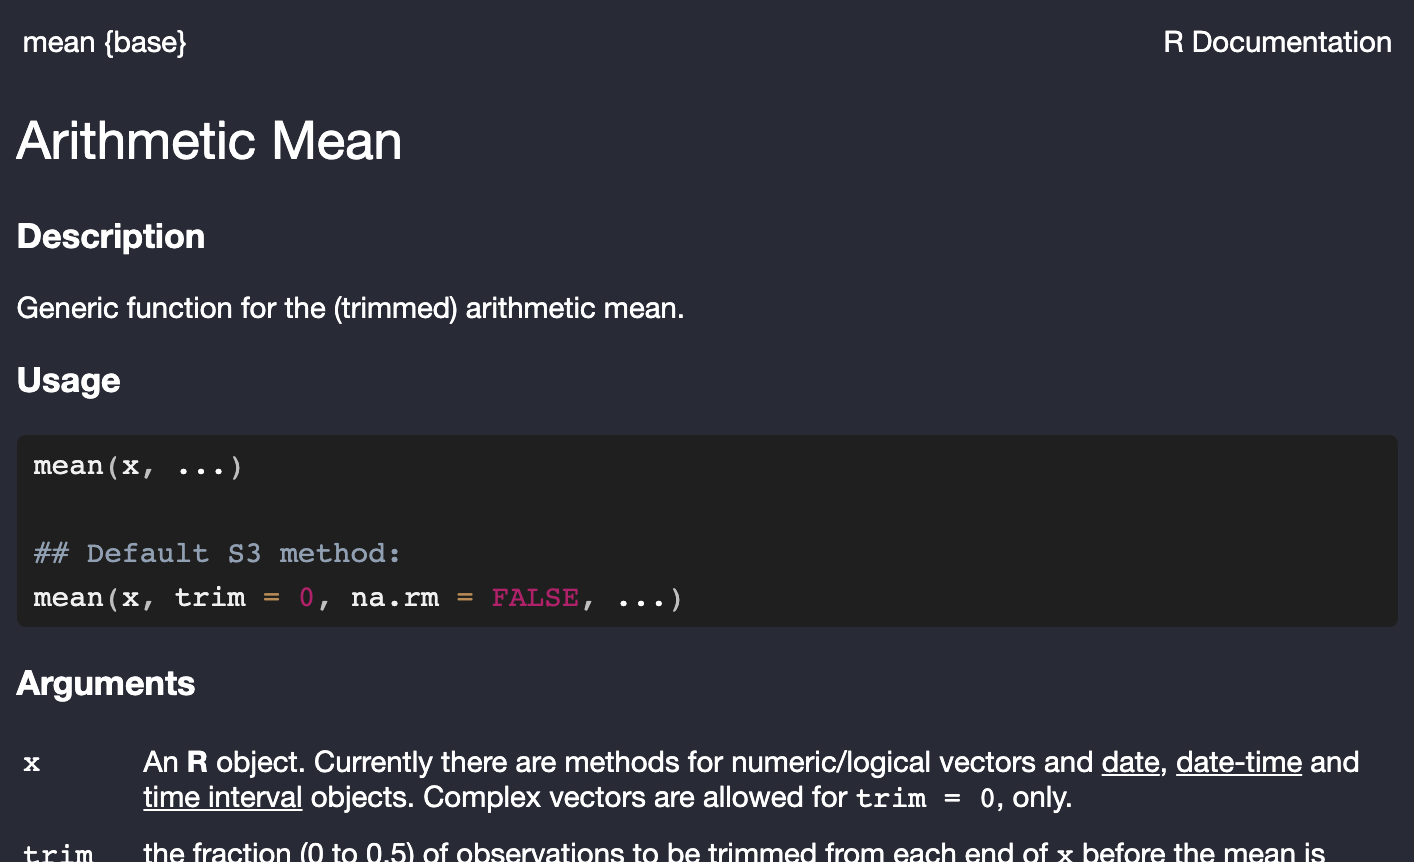
\includegraphics{Programmeren/figuren/Screenshot 2024-07-20 at 17.58.11.png}

}

\caption{Elephant}

\end{figure}%

\section{Zelf functies maken}\label{zelf-functies-maken}

Het handige aan functies is dat je ze ook zelf kan maken, als je
bijvoorbeeld iets heel specifieks wil doen. Je moet hiervoor aangeven
wat de argumenten zijn, welke berekening op basis van deze argumenten
wordt uitgevoerd, en wat er door de functie wordt teruggegeven (de
return-waarde). Hier is een voorbeeld:

\begin{Shaded}
\begin{Highlighting}[]
\CommentTok{\# Definitie van de functie}
\NormalTok{som\_kwadraten }\OtherTok{\textless{}{-}} \ControlFlowTok{function}\NormalTok{(a, b) \{}
\NormalTok{  resultaat }\OtherTok{\textless{}{-}}\NormalTok{ a}\SpecialCharTok{\^{}}\DecValTok{2} \SpecialCharTok{+}\NormalTok{ b}\SpecialCharTok{\^{}}\DecValTok{2}
  \FunctionTok{return}\NormalTok{(resultaat)}
\NormalTok{\}}

\CommentTok{\# Voorbeeld gebruik van de functie}
\FunctionTok{som\_kwadraten}\NormalTok{(}\DecValTok{1}\NormalTok{,}\DecValTok{2}\NormalTok{)            }\CommentTok{\# 5}
\FunctionTok{som\_kwadraten}\NormalTok{(}\DecValTok{3}\NormalTok{, }\DecValTok{4}\NormalTok{)           }\CommentTok{\# 25}
\FunctionTok{som\_kwadraten}\NormalTok{(}\FloatTok{0.5}\NormalTok{, }\FloatTok{0.1}\NormalTok{)       }\CommentTok{\# 0.26}
\end{Highlighting}
\end{Shaded}

\section{Condities}\label{condities}

Vaak is het handig om in een script te controleren of aan een bepaalde
voorwaarde wordt voldaan. Hiervoor kun je \texttt{if}, \texttt{else}, en
\texttt{else\ if} gebruiken:

\begin{Shaded}
\begin{Highlighting}[]
\NormalTok{leeftijd\_student }\OtherTok{\textless{}{-}} \FunctionTok{sample}\NormalTok{(}\DecValTok{16}\SpecialCharTok{:}\DecValTok{19}\NormalTok{,}\DecValTok{1}\NormalTok{)}
\NormalTok{volwassen\_leeftijd }\OtherTok{\textless{}{-}} \DecValTok{18}
\ControlFlowTok{if}\NormalTok{(leeftijd\_student }\SpecialCharTok{\textgreater{}=}\NormalTok{ volwassen\_leeftijd)\{}
  \FunctionTok{print}\NormalTok{(}\StringTok{"Student is volwassen"}\NormalTok{)}
\NormalTok{\} }\ControlFlowTok{else}\NormalTok{\{}
  \FunctionTok{print}\NormalTok{(}\StringTok{"Student is niet volwassen"}\NormalTok{)}
\NormalTok{\}}
\end{Highlighting}
\end{Shaded}

Om voorwaarden te controleren, gebruik je zoheten \textbf{conditionals},
die teruggeven of iets waar (\texttt{TRUE}) of niet waar
(\texttt{FALSE}) is. Hierboven gebruiken we \texttt{\textgreater{}=}
(groter dan of gelijk aan) om te controleren of de student minstens 18
jaar oud is. Veelgebruikte andere conditionals zijn:

\begin{itemize}
\tightlist
\item
  \texttt{a\ ==\ b} : TRUE als a gelijk is aan b
\end{itemize}

\begin{itemize}
\item
  \texttt{a\ !=\ b} : TRUE als a niet gelijk is aan b
\item
  \texttt{a\ \textgreater{}\ b} : TRUE als a is groter is dan b
\item
  \texttt{a\ \textless{}\ b} : TRUE als a is kleiner is dan b
\item
  \texttt{a\ \textgreater{}=\ b} : TRUE als a is groter is dan of gelijk
  is aan b
\item
  \texttt{a\ \textless{}=\ b} : TRUE als a is kleiner is dan of gelijk
  is aan b
\end{itemize}

Daarnaast kun je eventueel meerdere condities combineren:

\begin{itemize}
\item
  \texttt{a==b\ \&\ b!=c} : TRUE als a gelijk is aan b en b
  \textbf{niet} gelijk is aan c
\item
  \texttt{a\textless{}b\ \textbar{}\ b\textgreater{}c} : TRUE als a
  kleiner is dan b en b groter is dan c
\end{itemize}

Als laatste kun je nog veel meer combinaties controleren door
\texttt{if}-\texttt{else} elkaar op te laten volgen en te nesten. Als we
bijvoorbeeld twee dobbelsteenworpen simuleren, kunnen we precies
controleren welke dobbelsteen hoger is dan 4, en een voor ieder scenario
een unieke uitkomst maken:

\begin{Shaded}
\begin{Highlighting}[]
\NormalTok{d1 }\OtherTok{\textless{}{-}} \FunctionTok{sample}\NormalTok{(}\DecValTok{1}\SpecialCharTok{:}\DecValTok{6}\NormalTok{,}\DecValTok{1}\NormalTok{) }\CommentTok{\# dobbelsteen 1}
\NormalTok{d2 }\OtherTok{\textless{}{-}} \FunctionTok{sample}\NormalTok{(}\DecValTok{1}\SpecialCharTok{:}\DecValTok{6}\NormalTok{,}\DecValTok{1}\NormalTok{) }\CommentTok{\# dobbelsteen 2}

\ControlFlowTok{if}\NormalTok{ (d1 }\SpecialCharTok{\textgreater{}} \DecValTok{4}\NormalTok{) \{}
  \ControlFlowTok{if}\NormalTok{ (d2 }\SpecialCharTok{\textgreater{}} \DecValTok{4}\NormalTok{) \{}
    \FunctionTok{print}\NormalTok{(}\StringTok{"d1 en d2 zijn hoger dan 4"}\NormalTok{)}
\NormalTok{  \} }\ControlFlowTok{else}\NormalTok{ \{}
    \FunctionTok{print}\NormalTok{(}\StringTok{"d1 is hoger dan 4, maar d2 niet"}\NormalTok{)}
\NormalTok{  \}}
\NormalTok{\} }\ControlFlowTok{else} \ControlFlowTok{if}\NormalTok{(d2 }\SpecialCharTok{\textgreater{}} \DecValTok{4}\NormalTok{) \{}
  \FunctionTok{print}\NormalTok{(}\StringTok{"d1 is niet hoger dan 4, maar d2 wel"}\NormalTok{)}
\NormalTok{\} }
\end{Highlighting}
\end{Shaded}

Let op: als je de bovenstaande code goed leest, zie je dat er helemaal
\textbf{niets} gebeurt als geen van beide dobbelstenen groter dan 4 is.

\section{Loops}\label{loops}

Hoewel functies het makkelijker maken om dezelfde berekening meerdere
keren uit te voeren, wat nu als je een functie 100 keer wil aanroepen?
Hebben we dan 100 regels nodig? Het antwoord is nee, want elke
programmeertaal heeft manieren om stukken code te herhalen. In R bestaan
veel verschillende manieren om dit te doen (\texttt{repeat},
\texttt{apply}, \texttt{while}), maar in deze introductie maken we
vooral kennis met de meest-gebruikte loop: de for-loop.

Laten we bijvoorbeeld de exponentiele afname van paracetamol in het
bloed beschrijven met een simpele simulatie. Iemand neemt 400 milligram
paracetamol in, wat ieder uur (ongeveer) met 70\% afneemt:

\begin{Shaded}
\begin{Highlighting}[]
\NormalTok{p }\OtherTok{\textless{}{-}} \DecValTok{400} \CommentTok{\# hoeveelheid paracetamol}
\NormalTok{d }\OtherTok{\textless{}{-}} \FloatTok{0.7} \CommentTok{\# afname (d van decay)}
\CommentTok{\# Herhaal iets 10 keer, waarbij \textquotesingle{}i\textquotesingle{} steeds met 1 toeneemt}
\ControlFlowTok{for}\NormalTok{(i }\ControlFlowTok{in} \DecValTok{1}\SpecialCharTok{:}\DecValTok{10}\NormalTok{)\{}
\NormalTok{  p }\OtherTok{\textless{}{-}}\NormalTok{ p}\SpecialCharTok{*}\NormalTok{d}
\NormalTok{\}}
\FunctionTok{cat}\NormalTok{(}\StringTok{\textquotesingle{}Na 10 uur is er\textquotesingle{}}\NormalTok{,p,}\StringTok{\textquotesingle{}milligram paracetamol in het bloed\textquotesingle{}}\NormalTok{) }\CommentTok{\# 11.299 mg}
\end{Highlighting}
\end{Shaded}

Wellicht willen we graag bijhouden hoeveel paracetamol er in elke stap
aanwezig was, zodat we dat na onze loop kunnen plotten. Om dit te doen,
kunnen we de \texttt{i} als index gebruiken om een vector te vullen:

\begin{Shaded}
\begin{Highlighting}[]
\NormalTok{p }\OtherTok{\textless{}{-}} \DecValTok{400} \CommentTok{\# hoeveelheid paracetamol}
\NormalTok{d }\OtherTok{\textless{}{-}} \FloatTok{0.7} \CommentTok{\# afname (d van decay)}
\CommentTok{\# Herhaal iets 10 keer, waarbij \textquotesingle{}i\textquotesingle{} steeds met 1 toeneemt}
\ControlFlowTok{for}\NormalTok{(i }\ControlFlowTok{in} \DecValTok{1}\SpecialCharTok{:}\DecValTok{10}\NormalTok{)\{}
\NormalTok{  p[i}\SpecialCharTok{+}\DecValTok{1}\NormalTok{] }\OtherTok{\textless{}{-}}\NormalTok{ p[i]}\SpecialCharTok{*}\NormalTok{d}
\NormalTok{\}}
\FunctionTok{plot}\NormalTok{(p, }\AttributeTok{type=}\StringTok{\textquotesingle{}o\textquotesingle{}}\NormalTok{)}
\end{Highlighting}
\end{Shaded}

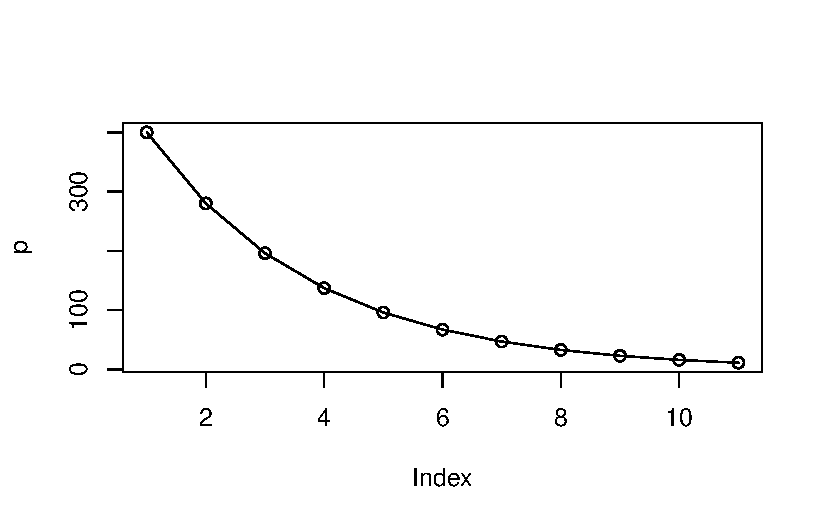
\includegraphics{Programmeren/intro_R_day2_files/figure-pdf/unnamed-chunk-17-1.pdf}

Omdat dit voorbeeld om simpele exponentiele afname gaat, hadden we de
bovenstaande berekening ook ``in één keer'' kunnen uitrekenen door
\$\(p \cdot d^{10}\)\$ uit te rekenen. Laten we dat even controleren:

\begin{Shaded}
\begin{Highlighting}[]
\NormalTok{p }\OtherTok{\textless{}{-}} \DecValTok{400} \CommentTok{\# hoeveelheid paracetamol}
\NormalTok{d }\OtherTok{\textless{}{-}} \FloatTok{0.7} \CommentTok{\# afname (d van decay)}
\NormalTok{p}\SpecialCharTok{*}\NormalTok{d}\SpecialCharTok{\^{}}\DecValTok{10} \CommentTok{\# 11.299 mg}
\end{Highlighting}
\end{Shaded}

Dit antwoord komt inderdaad overeen met onze berekening met de
\texttt{for} loop. Hoewel deze loop dus misschien wat onnodig lijkt,
hebben we niet altijd zo'n simpele formule beschikbaar. Bovendien willen
we wellicht iets veel specifiekers simuleren, bijvoorbeeld dat de
persoon elke 12 uur opnieuw paracetamol inneemt:

\begin{Shaded}
\begin{Highlighting}[]
\NormalTok{p }\OtherTok{\textless{}{-}} \DecValTok{400} \CommentTok{\# hoeveelheid paracetamol}
\NormalTok{d }\OtherTok{\textless{}{-}} \FloatTok{0.7} \CommentTok{\# afname (d van decay)}

\ControlFlowTok{for}\NormalTok{(i }\ControlFlowTok{in} \DecValTok{1}\SpecialCharTok{:}\DecValTok{100}\NormalTok{)\{}
  \ControlFlowTok{if}\NormalTok{(i}\SpecialCharTok{\%\%}\DecValTok{12}\SpecialCharTok{==}\DecValTok{0}\NormalTok{)\{ }\CommentTok{\# is i precies deelbaar door 12?}
\NormalTok{    p[i] }\OtherTok{\textless{}{-}}\NormalTok{ p[i] }\SpecialCharTok{+} \DecValTok{400}
\NormalTok{  \} }
\NormalTok{  p[i}\SpecialCharTok{+}\DecValTok{1}\NormalTok{] }\OtherTok{\textless{}{-}}\NormalTok{ p[i]}\SpecialCharTok{*}\NormalTok{d}
\NormalTok{\}}
\FunctionTok{plot}\NormalTok{(p, }\AttributeTok{type=}\StringTok{\textquotesingle{}o\textquotesingle{}}\NormalTok{)}
\end{Highlighting}
\end{Shaded}

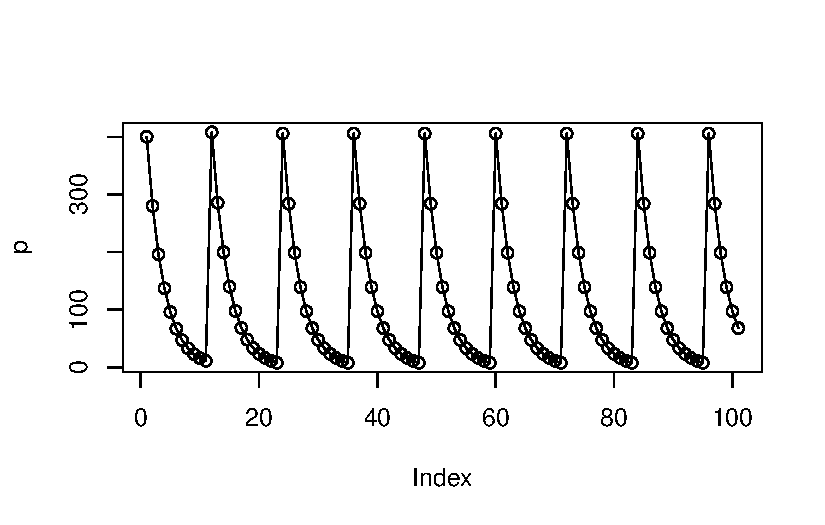
\includegraphics{Programmeren/intro_R_day2_files/figure-pdf/unnamed-chunk-19-1.pdf}

Of dat de persoon met 10\% kans elk uur een paracetamol inneemt:

\begin{Shaded}
\begin{Highlighting}[]
\NormalTok{p }\OtherTok{\textless{}{-}} \DecValTok{400} \CommentTok{\# hoeveelheid paracetamol}
\NormalTok{d }\OtherTok{\textless{}{-}} \FloatTok{0.7} \CommentTok{\# afname (d van decay)}

\ControlFlowTok{for}\NormalTok{(i }\ControlFlowTok{in} \DecValTok{1}\SpecialCharTok{:}\DecValTok{100}\NormalTok{)\{}
  \ControlFlowTok{if}\NormalTok{(}\FunctionTok{runif}\NormalTok{(}\DecValTok{1}\NormalTok{)}\SpecialCharTok{\textless{}}\FloatTok{0.1}\NormalTok{)\{ }\CommentTok{\# is willekeurig getal (tussen 0 en 1) kleiner dan 0.1?}
\NormalTok{    p[i] }\OtherTok{\textless{}{-}}\NormalTok{ p[i] }\SpecialCharTok{+} \DecValTok{400}
\NormalTok{  \} }
\NormalTok{  p[i}\SpecialCharTok{+}\DecValTok{1}\NormalTok{] }\OtherTok{\textless{}{-}}\NormalTok{ p[i]}\SpecialCharTok{*}\NormalTok{d}
\NormalTok{\}}
\FunctionTok{plot}\NormalTok{(p, }\AttributeTok{type=}\StringTok{\textquotesingle{}o\textquotesingle{}}\NormalTok{)}
\end{Highlighting}
\end{Shaded}

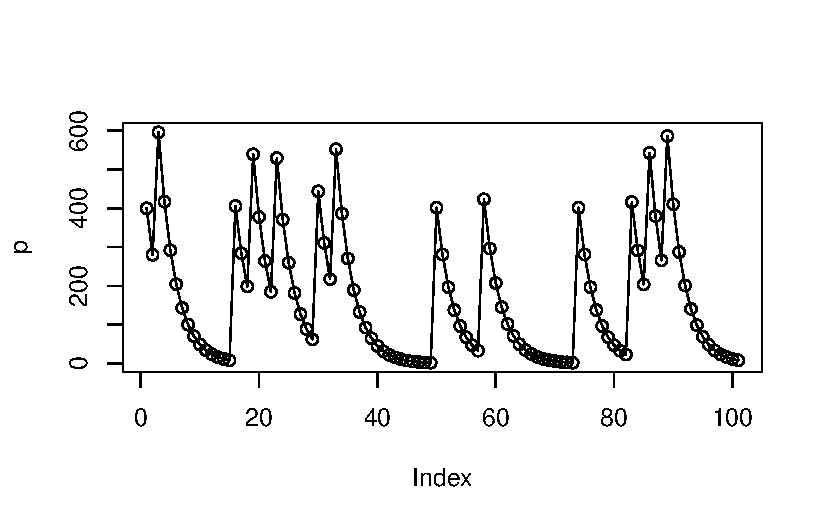
\includegraphics{Programmeren/intro_R_day2_files/figure-pdf/unnamed-chunk-20-1.pdf}

\chapter{Grafieken plotten met R}\label{grafieken-plotten-met-r}

Om de bovenstaande plot van de paracetamol afname iets vollediger en
mooier te maken, kunnen we meer argumenten aan de plotfunctie toevoegen:

\begin{Shaded}
\begin{Highlighting}[]
\NormalTok{p }\OtherTok{\textless{}{-}} \DecValTok{400} \CommentTok{\# hoeveelheid paracetamol}
\NormalTok{d }\OtherTok{\textless{}{-}} \FloatTok{0.7} \CommentTok{\# afname (d van decay)}

\ControlFlowTok{for}\NormalTok{(i }\ControlFlowTok{in} \DecValTok{1}\SpecialCharTok{:}\DecValTok{100}\NormalTok{)\{}
  \ControlFlowTok{if}\NormalTok{(}\FunctionTok{runif}\NormalTok{(}\DecValTok{1}\NormalTok{)}\SpecialCharTok{\textless{}}\FloatTok{0.1}\NormalTok{)\{ }\CommentTok{\# is willekeurig getal (tussen 0 en 1) kleiner dan 0.1?}
\NormalTok{    p[i] }\OtherTok{\textless{}{-}}\NormalTok{ p[i] }\SpecialCharTok{+} \DecValTok{400}
\NormalTok{  \} }
\NormalTok{  p[i}\SpecialCharTok{+}\DecValTok{1}\NormalTok{] }\OtherTok{\textless{}{-}}\NormalTok{ p[i]}\SpecialCharTok{*}\NormalTok{d}
\NormalTok{\}}
\FunctionTok{plot}\NormalTok{(p, }\AttributeTok{type=}\StringTok{\textquotesingle{}l\textquotesingle{}}\NormalTok{, }\AttributeTok{lwd=}\DecValTok{2}\NormalTok{, }\AttributeTok{col=}\StringTok{"purple"}\NormalTok{, }\AttributeTok{xlab=}\StringTok{"Tijd (uren)"}\NormalTok{, }\AttributeTok{ylab=}\StringTok{"Paracetamol in bloed"}\NormalTok{)}
\FunctionTok{legend}\NormalTok{(}\DecValTok{70}\NormalTok{, }\FunctionTok{max}\NormalTok{(p), }\AttributeTok{legend=}\FunctionTok{c}\NormalTok{(}\StringTok{"Paracetamol"}\NormalTok{), }\AttributeTok{col=}\FunctionTok{c}\NormalTok{(}\StringTok{"purple"}\NormalTok{),}\AttributeTok{lty=}\DecValTok{1}\NormalTok{,}\AttributeTok{lwd=}\DecValTok{2}\NormalTok{)}
\end{Highlighting}
\end{Shaded}

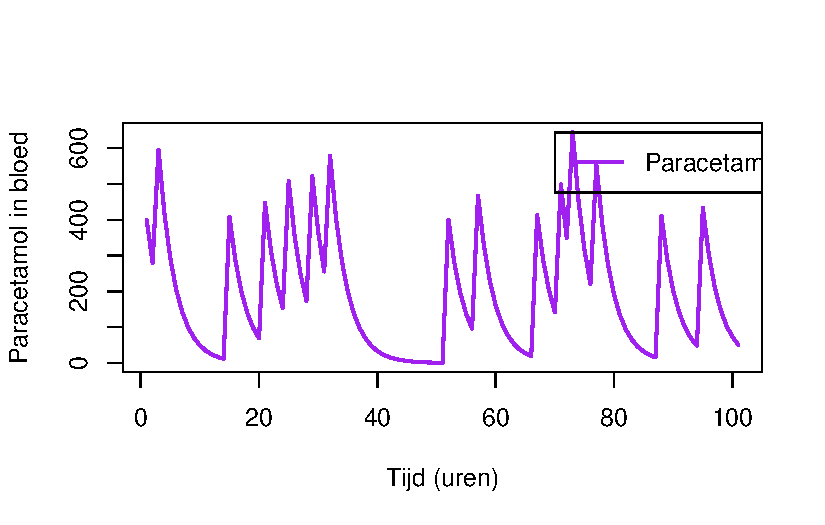
\includegraphics{Programmeren/intro_R_day2_files/figure-pdf/unnamed-chunk-21-1.pdf}

Er zijn binnen R nog veel meer manieren om data te plotten, zoals
bijvoorbeeld de \texttt{boxplot} die je bij het onderdeel statistiek
zeker nog tegen zal komen. Daarnaast zijn er in R veel \texttt{packages}
beschikbaar kunnen helpen bij het maken van mooie grafieken, zoals
\href{https://ggplot2.tidyverse.org/}{ggplot} maar daar gaan we in deze
cursus niet dieper op in.

\subsection{Opgaven deel 2: TODO}\label{opgaven-deel-2-todo}

\begin{enumerate}
\def\labelenumi{\arabic{enumi}.}
\tightlist
\item
  Neem bovenstaande script over in R (tip: je kan de hele code in 1 keer
  kopiëren met het knopje rechtsboven)
\item
  Voeg aan het einde van een script een extra regel toe, waar je de
  variabele \texttt{e} in \texttt{2} verandert.
\item
  Voer het script uit. De waarde van de uitkomst-variabele is niet
  verandert. Leg met de kook-analogie uit waarom niet.
\end{enumerate}

\chapter{Wat moet ik weten over R?}\label{wat-moet-ik-weten-over-r}

\begin{enumerate}
\def\labelenumi{\arabic{enumi}.}
\item
  Wat is het verschil tussen een matrix in een data frame\\
  A: matrix kan alleen dezelfde waarden bevatten, data frame kan (per
  kolom) verschillende type data bevatten.
\item
  \texttt{x\ \textless{}-\ seq(1,10,by=0.5)}

  Wat geeft x{[}2{]} ?\\
  opties (\textbf{1}, 0.5, 2, NA)
\item
  \texttt{x\ \textless{}-\ 10:1}

  Wat geeft x{[}1{]} ?\\
  antwoord = 10
\item
  x \textless- runif(10)
\item
  Wat geeft x{[}11{]}\\
  antwoord = NA
\item
  Beschouw hetvolgende data frame:

  \texttt{df\ \textless{}-\ data.frame(\ \ \ Naam\ =\ c("Jaap",\ "Alina",\ "Xin"),\ \ \ Minuten\ =\ c(12,\ 19,\ 11),\ \ \ Score\ =\ c(85,\ 90,\ 95)}

  \texttt{)}

  Stel we willen een nieuwe kolom toevoegen die de score per minuut
  geeft, wat moeten we daarvoor doen?\\
  A (goede):
  \texttt{df\$score\_per\_minuut\ \textless{}-\ df\$score/df\$minuten}A
  (fout): \texttt{df\$score\ \textless{}-\ df\$score/df\$minuten}A
  (fout):
  \texttt{df{[}score\_per\_minuut{]}\ \textless{}-\ df\$score/df\$minuten}A
  (fout):
  \texttt{df\ +\ score\_per\_minuut\ \textless{}-\ df\$score/df\$minutenA\ (fout):\ df\$score\_per\_minuut\ \textless{}-\ "score\ per\ minuut"}
\item
  Een student leest de volgende csv in van dieren in het asiel onder de
  naam ``dieren'':\\
  (iets met comma-separated values)\\
  \strut \\
  Naam, Leeftijd, Vachtkleur, Temperament\\
  Joey, 8, zwart, rustig\\
  \strut \\
  Niem, 2, wit, energiek\\
  Bob, 4, bruin, vriendelijk\\
  Saartje, 2, gevlekt, verlegen\\
  \strut \\
  dieren{[}2,3:4{]} geeft:\\
  \textbf{``wit'' en ``energiek''\\
  }''zwart'' en ``rustig''\\
  4 en 2\\
  4 en ``bruin''\\
  2 en ``wit''\\
  ``verlegen'' en ``gevlekt''\\
  8 en ``zwart''
\item
  Een for-loop met wat uitkmost afhankelijk van een if/else statement.
\item
\end{enumerate}

\part{Basiswiskunde}

\begin{figure}

\centering{


\includegraphics{Wiskunde/figuren/AI_mathematics.jpeg}

}

\caption{\label{fig-AI_mathematics}Wiskunde in de biologie; illustratie
gegenereerd door AI. (DALL-E 3, maart 2024)}

\end{figure}%

\chapter{Breuken}\label{breuken}

\chapter{Exponenten}\label{exponenten}

\chapter{Logaritmen}\label{logaritmen}

\chapter{Vergelijkingen oplossen}\label{vergelijkingen-oplossen}

\chapter{Limieten en asymptoten}\label{limieten-en-asymptoten}

\chapter{Schetsen}\label{schetsen}

\chapter{Afgeleiden}\label{afgeleiden}

\bookmarksetup{startatroot}

\chapter{Voorbeelden van wat mogelijk is met
Quarto}\label{voorbeelden-van-wat-mogelijk-is-met-quarto}

\usepackage{libertine}
\addtokomafont{disposition}{\rmfamily}
\renewcommand{\ttdefault}{clmt}

\providecommand{\ped}[1]{_\textrm{#1}}
\providecommand{\ap}[1]{^\textrm{#1}}
\providecommand{\app}[1]{^\textrm{#1}}

\providecommand*{\angs}{\smash{\mathrm{\ring A}}}
\providecommand*{\celsius}{\mathrm{~\circ C}}
\providecommand*{\micro}{\mu}

\providecommand*{\unit}[1]{\textrm{\,#1}}

\providecommand{\E}{\mathrm{e}}
\providecommand{\I}{\mathrm{i}}
\providecommand{\sfrac}[2]{^{#1}/_{#2}}

\providecommand{\conc}[1]{\left[\mathrm{#1}\right]}

\providecommand{\command}[1]{\textsl{#1}}
\providecommand{\out}[1]{\begin{verbatim}#1\end{verbatim}}

\providecommand{\diff}{\mathrm{d}\,}

\providecommand*{\deriv}[3][]{% arguments: order of the derivative(optional), function, variable
    \frac{\diff^{#1}#2}{\diff #3^{#1}}}
\providecommand*{\pderiv}[3][]{% arguments: order of the derivative(optional), function, variable
    \frac{\partial^{#1}#2}
        {\partial #3^{#1}}}

\renewcommand{\vec}[1]{{\boldsymbol #1}}

\providecommand{\cov}[2]{\mathrm{Cov}\!\left(#1, #2\right)}
\providecommand{\var}[1]{\mathrm{Var}\!\left(#1\right)}

\providecommand{\mean}[1]{\overline{#1}}

\providecommand{\sd}[1]{\sigma\left(#1\right)}
\providecommand{\ev}[1]{\mathbb{E}\!\left(#1\right)}
\providecommand{\pr}[1]{\textrm{Pr}\!\left(#1\right)}

\section{Hoofdstuk}\label{hoofdstuk}

\subsection{Paragraaf binnen
hoofdstukje}\label{paragraaf-binnen-hoofdstukje}

\subsection{Plotjes maken in R}\label{plotjes-maken-in-r}

\begin{Shaded}
\begin{Highlighting}[]
\FunctionTok{library}\NormalTok{(ggplot2)}
\FunctionTok{library}\NormalTok{(tidyverse)}

\NormalTok{z\_values }\OtherTok{\textless{}{-}} \FunctionTok{seq}\NormalTok{(}\SpecialCharTok{{-}}\DecValTok{3}\NormalTok{, }\DecValTok{3}\NormalTok{, }\AttributeTok{by =} \FloatTok{0.01}\NormalTok{)}
\NormalTok{probabilities }\OtherTok{\textless{}{-}} \FunctionTok{dnorm}\NormalTok{(z\_values)}

\NormalTok{df }\OtherTok{\textless{}{-}} \FunctionTok{data.frame}\NormalTok{(}\AttributeTok{Z =}\NormalTok{ z\_values, }\AttributeTok{probability =}\NormalTok{ probabilities)}

\NormalTok{arrows }\OtherTok{\textless{}{-}} \FunctionTok{tibble}\NormalTok{(}
  \AttributeTok{x1 =} \FunctionTok{c}\NormalTok{(}\FloatTok{2.2}\NormalTok{), }
  \AttributeTok{x2 =} \FunctionTok{c}\NormalTok{(}\FloatTok{3.3}\NormalTok{),}
  \AttributeTok{y1 =} \FunctionTok{c}\NormalTok{(.}\DecValTok{02}\NormalTok{),}
  \AttributeTok{y2 =} \FunctionTok{c}\NormalTok{(}\FloatTok{0.15}\NormalTok{)}
\NormalTok{)}

\NormalTok{p }\OtherTok{\textless{}{-}} \FunctionTok{ggplot}\NormalTok{(df, }\FunctionTok{aes}\NormalTok{(}\AttributeTok{x =}\NormalTok{ Z, }\AttributeTok{y =}\NormalTok{ probability)) }\SpecialCharTok{+}
  \FunctionTok{geom\_line}\NormalTok{(}
    \AttributeTok{size =} \FloatTok{1.2}\NormalTok{,}
    \AttributeTok{color =} \StringTok{"\#e8601d"}
\NormalTok{    ) }\SpecialCharTok{+}
  \FunctionTok{geom\_ribbon}\NormalTok{(}
    \AttributeTok{data =} \FunctionTok{subset}\NormalTok{(df, Z }\SpecialCharTok{\textgreater{}=} \FloatTok{1.96}\NormalTok{), }
    \FunctionTok{aes}\NormalTok{(}\AttributeTok{ymax =}\NormalTok{ probability, }\AttributeTok{ymin =} \DecValTok{0}\NormalTok{), }
    \AttributeTok{fill =} \StringTok{"goldenrod"}\NormalTok{, }
    \AttributeTok{alpha =} \FloatTok{0.5}\NormalTok{) }\SpecialCharTok{+}
  \FunctionTok{geom\_vline}\NormalTok{(}
    \AttributeTok{xintercept =} \FloatTok{1.96}\NormalTok{, }
    \AttributeTok{linetype =} \StringTok{"dashed"}\NormalTok{, }
    \AttributeTok{color =} \StringTok{"black"}
\NormalTok{    ) }\SpecialCharTok{+}
  \FunctionTok{geom\_text}\NormalTok{(}
    \AttributeTok{x =} \FloatTok{0.6}\NormalTok{, }\AttributeTok{y =} \FloatTok{0.04}\NormalTok{, }
    \AttributeTok{label =} \FunctionTok{expression}\NormalTok{(}\FunctionTok{italic}\NormalTok{(Z)[}\FloatTok{0.05}\NormalTok{] }\SpecialCharTok{==} \FloatTok{1.96}\NormalTok{), }
    \AttributeTok{color =} \StringTok{"black"}\NormalTok{, }
    \AttributeTok{size =} \DecValTok{5}\NormalTok{,}
    \AttributeTok{parse =} \ConstantTok{TRUE}\NormalTok{, }
    \AttributeTok{hjust =} \SpecialCharTok{{-}}\FloatTok{0.2}\NormalTok{) }\SpecialCharTok{+}
  \FunctionTok{geom\_label}\NormalTok{(}
    \AttributeTok{x =} \FloatTok{2.4}\NormalTok{, }\AttributeTok{y =} \FloatTok{0.17}\NormalTok{, }
    \AttributeTok{label =} \FunctionTok{expression}\NormalTok{(alpha }\SpecialCharTok{==} \FloatTok{0.05}\NormalTok{), }
    \AttributeTok{color =} \StringTok{"black"}\NormalTok{, }
    \AttributeTok{fill =} \StringTok{"goldenrod"}\NormalTok{,}
    \AttributeTok{alpha =} \FloatTok{0.1}\NormalTok{,}
    \AttributeTok{label.size =} \DecValTok{0}\NormalTok{,}
    \AttributeTok{size =} \DecValTok{5}\NormalTok{,}
    \AttributeTok{parse =} \ConstantTok{TRUE}\NormalTok{, }
    \AttributeTok{hjust =} \SpecialCharTok{{-}}\FloatTok{0.2}\NormalTok{) }\SpecialCharTok{+}
  \FunctionTok{labs}\NormalTok{(}
       \AttributeTok{x =} \FunctionTok{expression}\NormalTok{(}\FunctionTok{italic}\NormalTok{(Z)),}
       \AttributeTok{y =} \StringTok{"probability density"}\NormalTok{,}
\NormalTok{       ) }\SpecialCharTok{+}
  \FunctionTok{geom\_curve}\NormalTok{(}
    \AttributeTok{data =}\NormalTok{ arrows, }
    \FunctionTok{aes}\NormalTok{(}\AttributeTok{x =}\NormalTok{ x1, }\AttributeTok{y =}\NormalTok{ y1, }\AttributeTok{xend =}\NormalTok{ x2, }\AttributeTok{yend =}\NormalTok{ y2),}
    \AttributeTok{arrow =} \FunctionTok{arrow}\NormalTok{(}
      \AttributeTok{length =} \FunctionTok{unit}\NormalTok{(}\FloatTok{0.1}\NormalTok{, }\StringTok{"inch"}\NormalTok{), }\AttributeTok{angle =} \DecValTok{30}\NormalTok{), }
    \AttributeTok{size =} \DecValTok{1}\NormalTok{,}
    \AttributeTok{color =} \StringTok{"gray30"}\NormalTok{, }
    \AttributeTok{curvature =} \FloatTok{0.4}
\NormalTok{    )}
\NormalTok{p}

\CommentTok{\#library(plotly)}
\CommentTok{\#ggplotly(p)}
\end{Highlighting}
\end{Shaded}

\begin{figure}[H]

\centering{

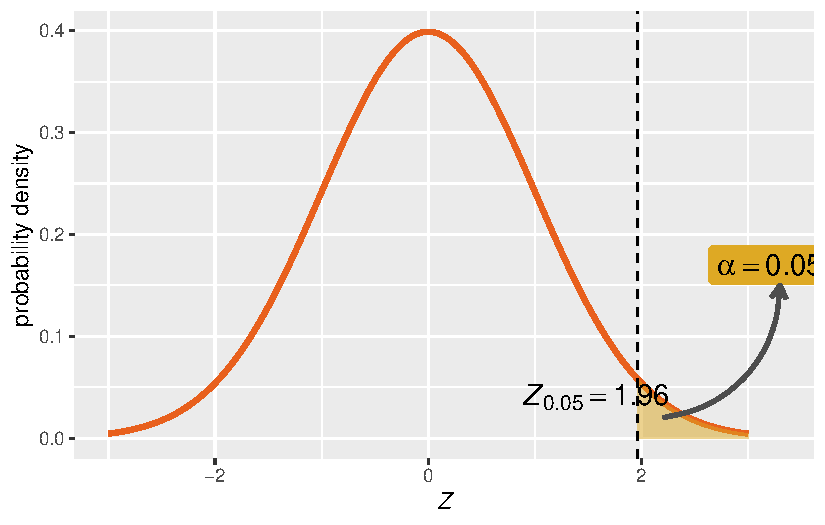
\includegraphics{voorbeelden_files/figure-pdf/fig-normal-1.pdf}

}

\caption{\label{fig-normal}Standard normal distribution with critical
value for \(\alpha = 0.05\).}

\end{figure}%

\begin{Shaded}
\begin{Highlighting}[]
\FunctionTok{library}\NormalTok{(ggplot2)}

\NormalTok{t\_values }\OtherTok{\textless{}{-}} \FunctionTok{seq}\NormalTok{(}\SpecialCharTok{{-}}\DecValTok{3}\NormalTok{, }\DecValTok{3}\NormalTok{, }\AttributeTok{by =} \FloatTok{0.1}\NormalTok{)}
\NormalTok{z\_values }\OtherTok{\textless{}{-}} \FunctionTok{seq}\NormalTok{(}\SpecialCharTok{{-}}\DecValTok{3}\NormalTok{, }\DecValTok{3}\NormalTok{, }\AttributeTok{by =} \FloatTok{0.1}\NormalTok{)}

\NormalTok{dataframe }\OtherTok{\textless{}{-}} \FunctionTok{data.frame}\NormalTok{(}
  \AttributeTok{t =} \FunctionTok{c}\NormalTok{(z\_values, }\FunctionTok{rep}\NormalTok{(t\_values, }\DecValTok{3}\NormalTok{)),}
  \AttributeTok{prob =} \FunctionTok{c}\NormalTok{(}
    \FunctionTok{dnorm}\NormalTok{(z\_values),}
    \FunctionTok{dt}\NormalTok{(t\_values, }\AttributeTok{df =} \DecValTok{1}\NormalTok{),}
    \FunctionTok{dt}\NormalTok{(t\_values, }\AttributeTok{df =} \DecValTok{5}\NormalTok{),}
    \FunctionTok{dt}\NormalTok{(t\_values, }\AttributeTok{df =} \DecValTok{20}\NormalTok{)}
\NormalTok{  ),}
  \AttributeTok{df =} \FunctionTok{factor}\NormalTok{(}
    \FunctionTok{c}\NormalTok{(}
      \FunctionTok{rep}\NormalTok{(}\StringTok{"standard normal"}\NormalTok{, }\FunctionTok{length}\NormalTok{(z\_values)),}
      \FunctionTok{rep}\NormalTok{(}\StringTok{"df = 1"}\NormalTok{, }\FunctionTok{length}\NormalTok{(t\_values)),}
      \FunctionTok{rep}\NormalTok{(}\StringTok{"df = 5"}\NormalTok{, }\FunctionTok{length}\NormalTok{(t\_values)),}
      \FunctionTok{rep}\NormalTok{(}\StringTok{"df = 20"}\NormalTok{, }\FunctionTok{length}\NormalTok{(t\_values))}
\NormalTok{      ),}
    \AttributeTok{levels =} \FunctionTok{c}\NormalTok{(}
      \StringTok{"df = 1"}\NormalTok{, }\StringTok{"df = 5"}\NormalTok{, }\StringTok{"df = 20"}\NormalTok{, }\StringTok{"standard normal"}
\NormalTok{      )}
\NormalTok{    ) }
\NormalTok{  )}

\FunctionTok{ggplot}\NormalTok{(}
\NormalTok{  dataframe, }
  \FunctionTok{aes}\NormalTok{(}
    \AttributeTok{x =}\NormalTok{ t, }\AttributeTok{y =}\NormalTok{ prob, }
    \AttributeTok{group =}\NormalTok{ df, }\AttributeTok{color =}\NormalTok{ df, }\AttributeTok{linewidth =}\NormalTok{ df, }\AttributeTok{linetype =}\NormalTok{ df)}
\NormalTok{  ) }\SpecialCharTok{+}
  \FunctionTok{geom\_line}\NormalTok{(}
\NormalTok{  ) }\SpecialCharTok{+}
  \FunctionTok{scale\_color\_manual}\NormalTok{(}
    \AttributeTok{values =} \FunctionTok{c}\NormalTok{( }\FunctionTok{rep}\NormalTok{(}\StringTok{"black"}\NormalTok{, }\DecValTok{3}\NormalTok{), }\StringTok{"\#e8601d"}\NormalTok{)}
\NormalTok{    ) }\SpecialCharTok{+} 
  \FunctionTok{scale\_linewidth\_manual}\NormalTok{(}
    \AttributeTok{values =} \FunctionTok{c}\NormalTok{(}\DecValTok{1}\NormalTok{, }\DecValTok{1}\NormalTok{, }\DecValTok{1}\NormalTok{, }\FloatTok{1.2}\NormalTok{)}
\NormalTok{  ) }\SpecialCharTok{+}
  \FunctionTok{scale\_linetype\_manual}\NormalTok{(}
    \AttributeTok{values =} \FunctionTok{c}\NormalTok{(}
      \StringTok{"df = 1"}\OtherTok{=}\StringTok{"longdash"}\NormalTok{, }
      \StringTok{"df = 5"}\OtherTok{=}\StringTok{"dashed"}\NormalTok{, }
      \StringTok{"df = 20"}\OtherTok{=}\StringTok{"dotted"}\NormalTok{,}
      \StringTok{"standard normal"}\OtherTok{=}\StringTok{"solid"} 
\NormalTok{    )}
\NormalTok{  ) }\SpecialCharTok{+}
  \FunctionTok{labs}\NormalTok{(}
    \AttributeTok{x =} \FunctionTok{expression}\NormalTok{(}\FunctionTok{italic}\NormalTok{(t)),}
    \AttributeTok{y =} \StringTok{"probability density"}
\NormalTok{  )}
\end{Highlighting}
\end{Shaded}

\begin{figure}[H]

\centering{

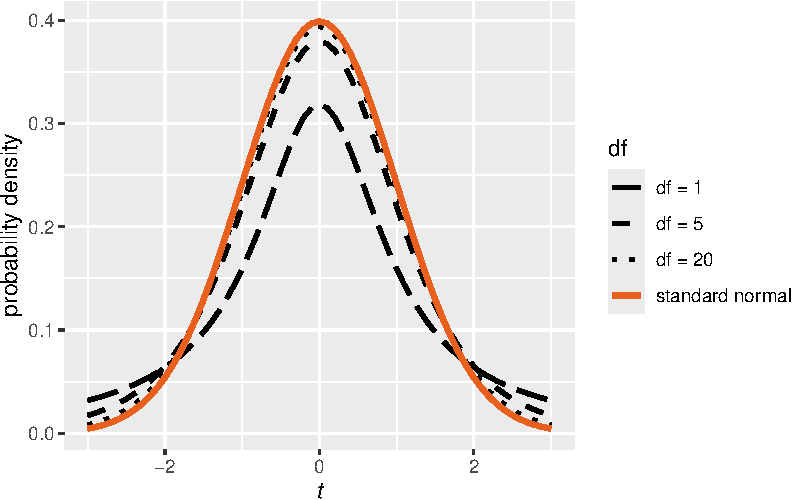
\includegraphics{voorbeelden_files/figure-pdf/fig-tdistributions-1.pdf}

}

\caption{\label{fig-tdistributions}Various \(t\)-distributions and a
normal distribution}

\end{figure}%

\#:::\{.content-visible when-format=``html''\}

\begin{Shaded}
\begin{Highlighting}[]
\FunctionTok{library}\NormalTok{(plotly)}
\NormalTok{p }\OtherTok{\textless{}{-}} \FunctionTok{qplot}\NormalTok{(}\FunctionTok{c}\NormalTok{(}\DecValTok{1}\NormalTok{, }\DecValTok{2}\NormalTok{, }\DecValTok{3}\NormalTok{), }\FunctionTok{c}\NormalTok{(}\DecValTok{4}\NormalTok{, }\DecValTok{2}\NormalTok{, }\DecValTok{4}\NormalTok{))}
\FunctionTok{ggplotly}\NormalTok{(p)}
\end{Highlighting}
\end{Shaded}

\begin{figure}[H]

\centering{

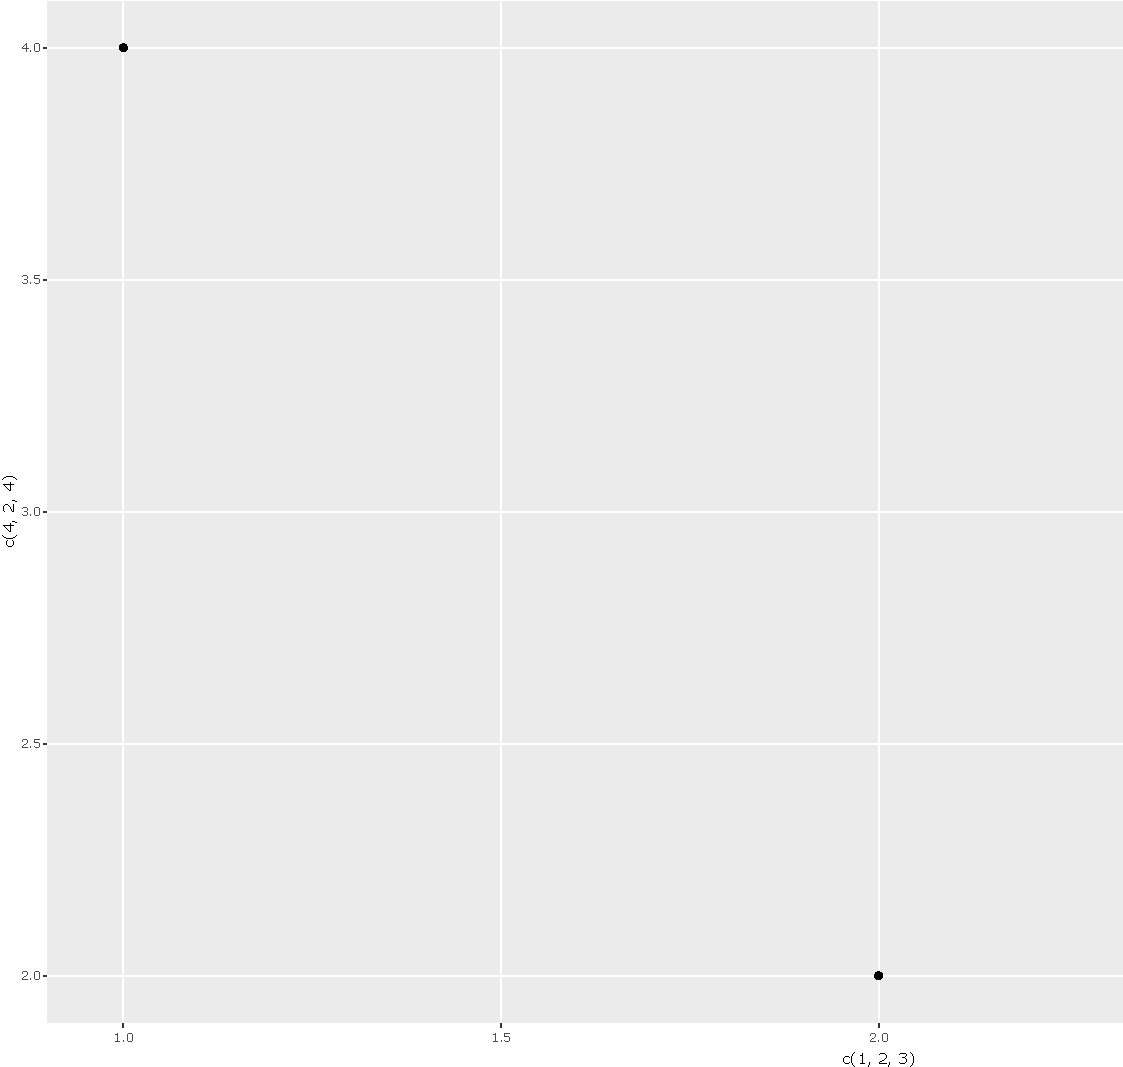
\includegraphics{voorbeelden_files/figure-pdf/fig-plotly-1.pdf}

}

\caption{\label{fig-plotly}test}

\end{figure}%

\#:::

\subsection{Inladen van een simulatie in Javascript die elders gehost
is}\label{inladen-van-een-simulatie-in-javascript-die-elders-gehost-is}

In de html-versie wordt dit getoond:

In de PDF-versie wordt dit getoond:

\begin{figure}[H]

{\centering 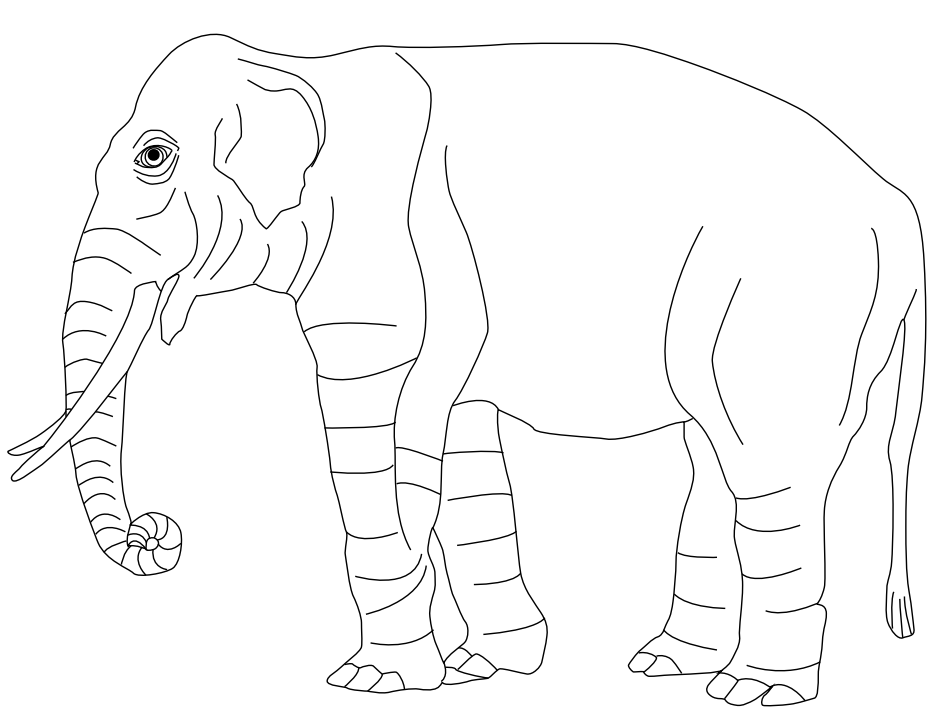
\includegraphics[width=4in,height=\textheight]{./figuren/elephant.png}

}

\caption{Ga naar \url{https://tbb.bio.uu.nl/bvd/simulations/australia/}
voor de simulatie.}

\end{figure}%

\subsection{LaTeX-macros}\label{latex-macros}

In het bestand \_macros.tex kunnen macros worden gedefinieerd. Dat
bestand moet bovenaan ieder document worden ingeladen (zie eerste regel
van dit bestand).

\subsection{Voorbeelden:}\label{voorbeelden}

Voor kansverdelingen heb ik de macro \textbackslash pr\{\}\$
gedefineerd:
\[\textrm{Pr}\!\left(A \cap B\right) = \textrm{Pr}\!\left(A\right) \textrm{Pr}\!\left(B | A\right).\]

\[\textrm{Pr}\!\left(A \cup B\right) = \textrm{Pr}\!\left(A\right) + \textrm{Pr}\!\left(B\right) - \textrm{Pr}\!\left(A \cap B\right).\]

Voor de verwachtingswaarde de macro \textbackslash ev\{\}: \[
\mathbb{E}\!\left(X\right) = \sum_x  x\, \textrm{Pr}\!\left(X = x\right).
\] De differentiaaloperator is \textbackslash diff: \[
\mathbb{E}\!\left(X\right) = \int_{-\infty}^\infty  x\, \textrm{Pr}\!\left(X = x\right)  \mathrm{d}\,x.
\] Voor varianties \textbackslash var\{\}``:

\[
\mathrm{Var}\!\left(X\right)  = \sum_x  \left(x - \mathbb{E}\!\left(X\right)\right)^2 \, \textrm{Pr}\!\left(X = x\right)
\] \[
\mathrm{Var}\!\left(X\right) = \int_{-\infty}^\infty  \left(x - \mathbb{E}\!\left(X\right)\right)^2 \, \textrm{Pr}\!\left(X = x\right) \mathrm{d}\,x.
\]

Voor standaarddeviaties \textbackslash sd\{\}: \[
\sigma\left(X\right) = \sqrt{\mathrm{Var}\!\left(X\right)}.
\]

\subsection{Mermaid}\label{mermaid}

Met Mermaid kun je heel gemakkelijk diagrammen maken:

\begin{figure}

\centering{

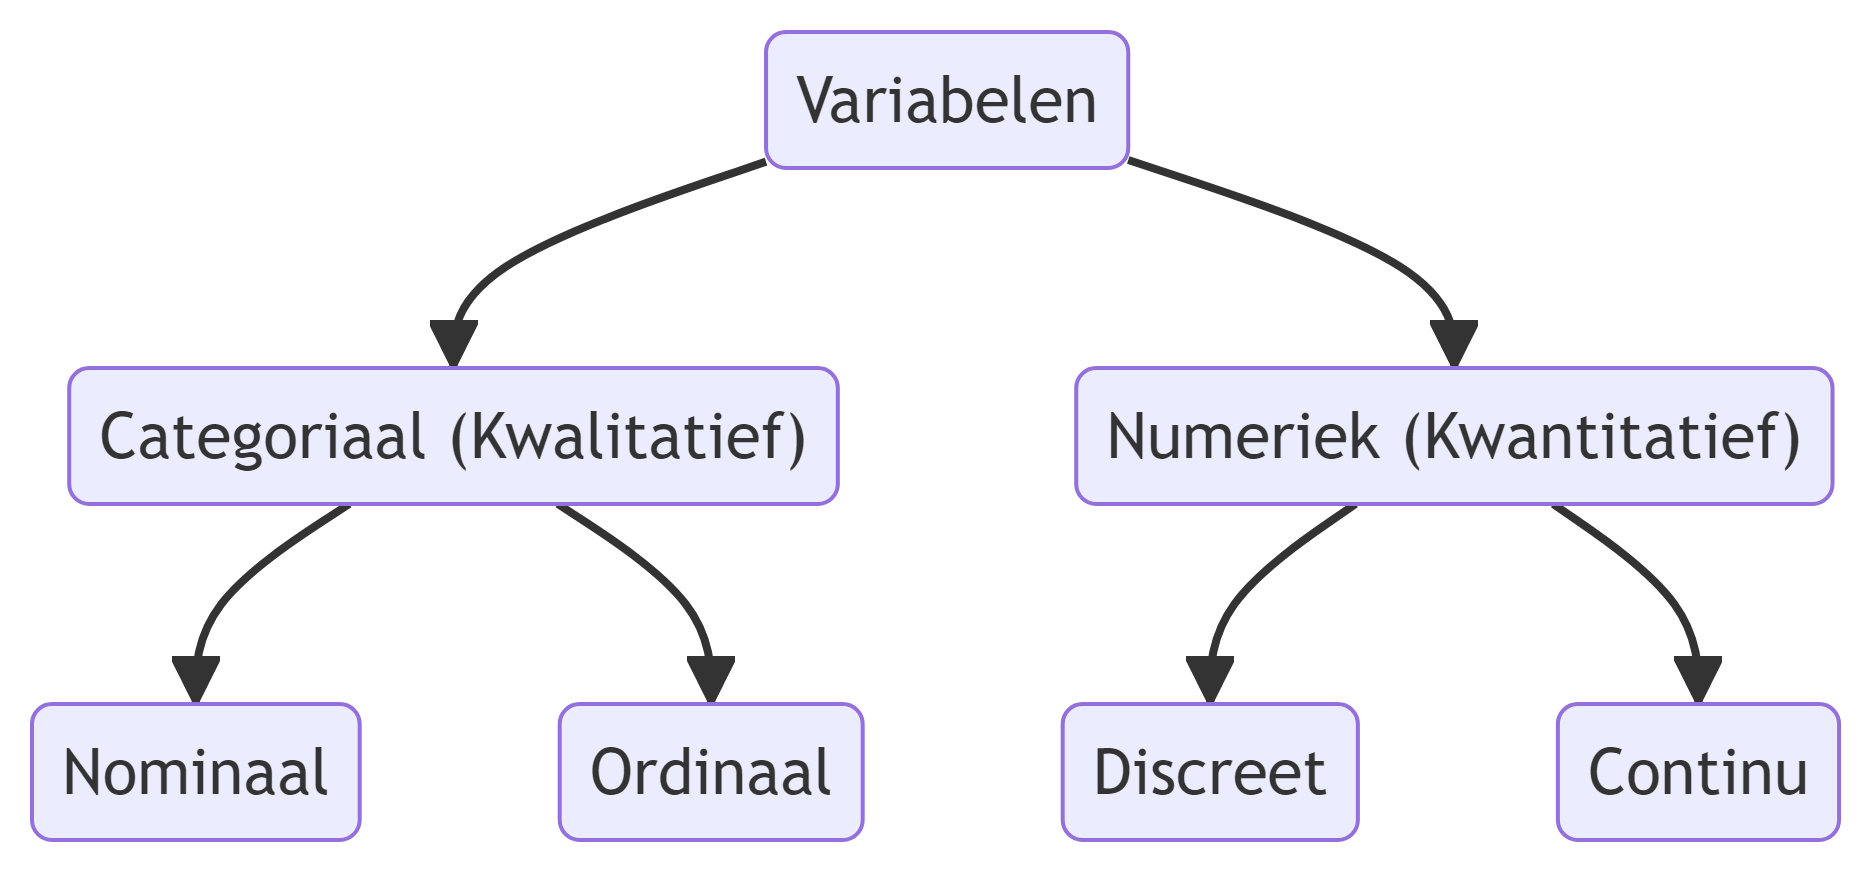
\includegraphics[width=4.87in,height=2.26in]{voorbeelden_files/figure-latex/mermaid-figure-1.png}

}

\caption{\label{fig-variables}}

\end{figure}%

\subsection{Callouts}\label{callouts}

We kunnen gebruik maken van call-outs:

\begin{tcolorbox}[enhanced jigsaw, coltitle=black, title=\textcolor{quarto-callout-note-color}{\faInfo}\hspace{0.5em}{Opmerking}, breakable, colframe=quarto-callout-note-color-frame, bottomtitle=1mm, opacityback=0, leftrule=.75mm, toptitle=1mm, titlerule=0mm, colback=white, toprule=.15mm, bottomrule=.15mm, arc=.35mm, rightrule=.15mm, colbacktitle=quarto-callout-note-color!10!white, opacitybacktitle=0.6, left=2mm]

Note that there are five types of callouts, including: \texttt{note},
\texttt{warning}, \texttt{important}, \texttt{tip}, and
\texttt{caution}.

\end{tcolorbox}

\begin{tcolorbox}[enhanced jigsaw, coltitle=black, title=\textcolor{quarto-callout-tip-color}{\faLightbulb}\hspace{0.5em}{Tip with Title}, breakable, colframe=quarto-callout-tip-color-frame, bottomtitle=1mm, opacityback=0, leftrule=.75mm, toptitle=1mm, titlerule=0mm, colback=white, toprule=.15mm, bottomrule=.15mm, arc=.35mm, rightrule=.15mm, colbacktitle=quarto-callout-tip-color!10!white, opacitybacktitle=0.6, left=2mm]

This is an example of a callout with a title.

\end{tcolorbox}

\begin{tcolorbox}[enhanced jigsaw, coltitle=black, title=\textcolor{quarto-callout-caution-color}{\faFire}\hspace{0.5em}{Expand To Learn About Collapse}, breakable, colframe=quarto-callout-caution-color-frame, bottomtitle=1mm, opacityback=0, leftrule=.75mm, toptitle=1mm, titlerule=0mm, colback=white, toprule=.15mm, bottomrule=.15mm, arc=.35mm, rightrule=.15mm, colbacktitle=quarto-callout-caution-color!10!white, opacitybacktitle=0.6, left=2mm]

This is an example of a `folded' caution callout that can be expanded by
the user. You can use \texttt{collapse="true"} to collapse it by default
or \texttt{collapse="false"} to make a collapsible callout that is
expanded by default.

\end{tcolorbox}

\begin{tcolorbox}[enhanced jigsaw, coltitle=black, title=\textcolor{quarto-callout-tip-color}{\faLightbulb}\hspace{0.5em}{Tip \ref*{tip-example}: Cross-Referencing a Tip}, breakable, colframe=quarto-callout-tip-color-frame, bottomtitle=1mm, opacityback=0, leftrule=.75mm, toptitle=1mm, titlerule=0mm, colback=white, toprule=.15mm, bottomrule=.15mm, arc=.35mm, rightrule=.15mm, colbacktitle=quarto-callout-tip-color!10!white, opacitybacktitle=0.6, left=2mm]

\quartocallouttip{tip-example} 

Add an ID starting with \texttt{\#tip-} to reference a tip.

\end{tcolorbox}

See Tip~\ref{tip-example}\ldots{}

\subsection{How to format questions/problem
sets}\label{how-to-format-questionsproblem-sets}

\begin{exercise}[Test
1]\protect\hypertarget{exr-test1}{}\label{exr-test1}

The equation of any straight line, called a linear equation, can be
written as:

\begin{equation}\phantomsection\label{eq-line}{ 
y = mx + b
}\end{equation}

Je kunt verwijzen naar Vergelijking~\ref{eq-line}, of
Verg.~\ref{eq-line}.

\textbf{a.} Blabla?

\textbf{b.} Of blablabla?

\end{exercise}

\subsection{Data Tables}\label{data-tables}

\begin{Shaded}
\begin{Highlighting}[]
\FunctionTok{library}\NormalTok{(DT)}
\FunctionTok{library}\NormalTok{(datasets)}
\FunctionTok{datatable}\NormalTok{(anscombe, }\AttributeTok{options =} \FunctionTok{list}\NormalTok{(}\AttributeTok{pageLength =} \DecValTok{5}\NormalTok{))}
\end{Highlighting}
\end{Shaded}

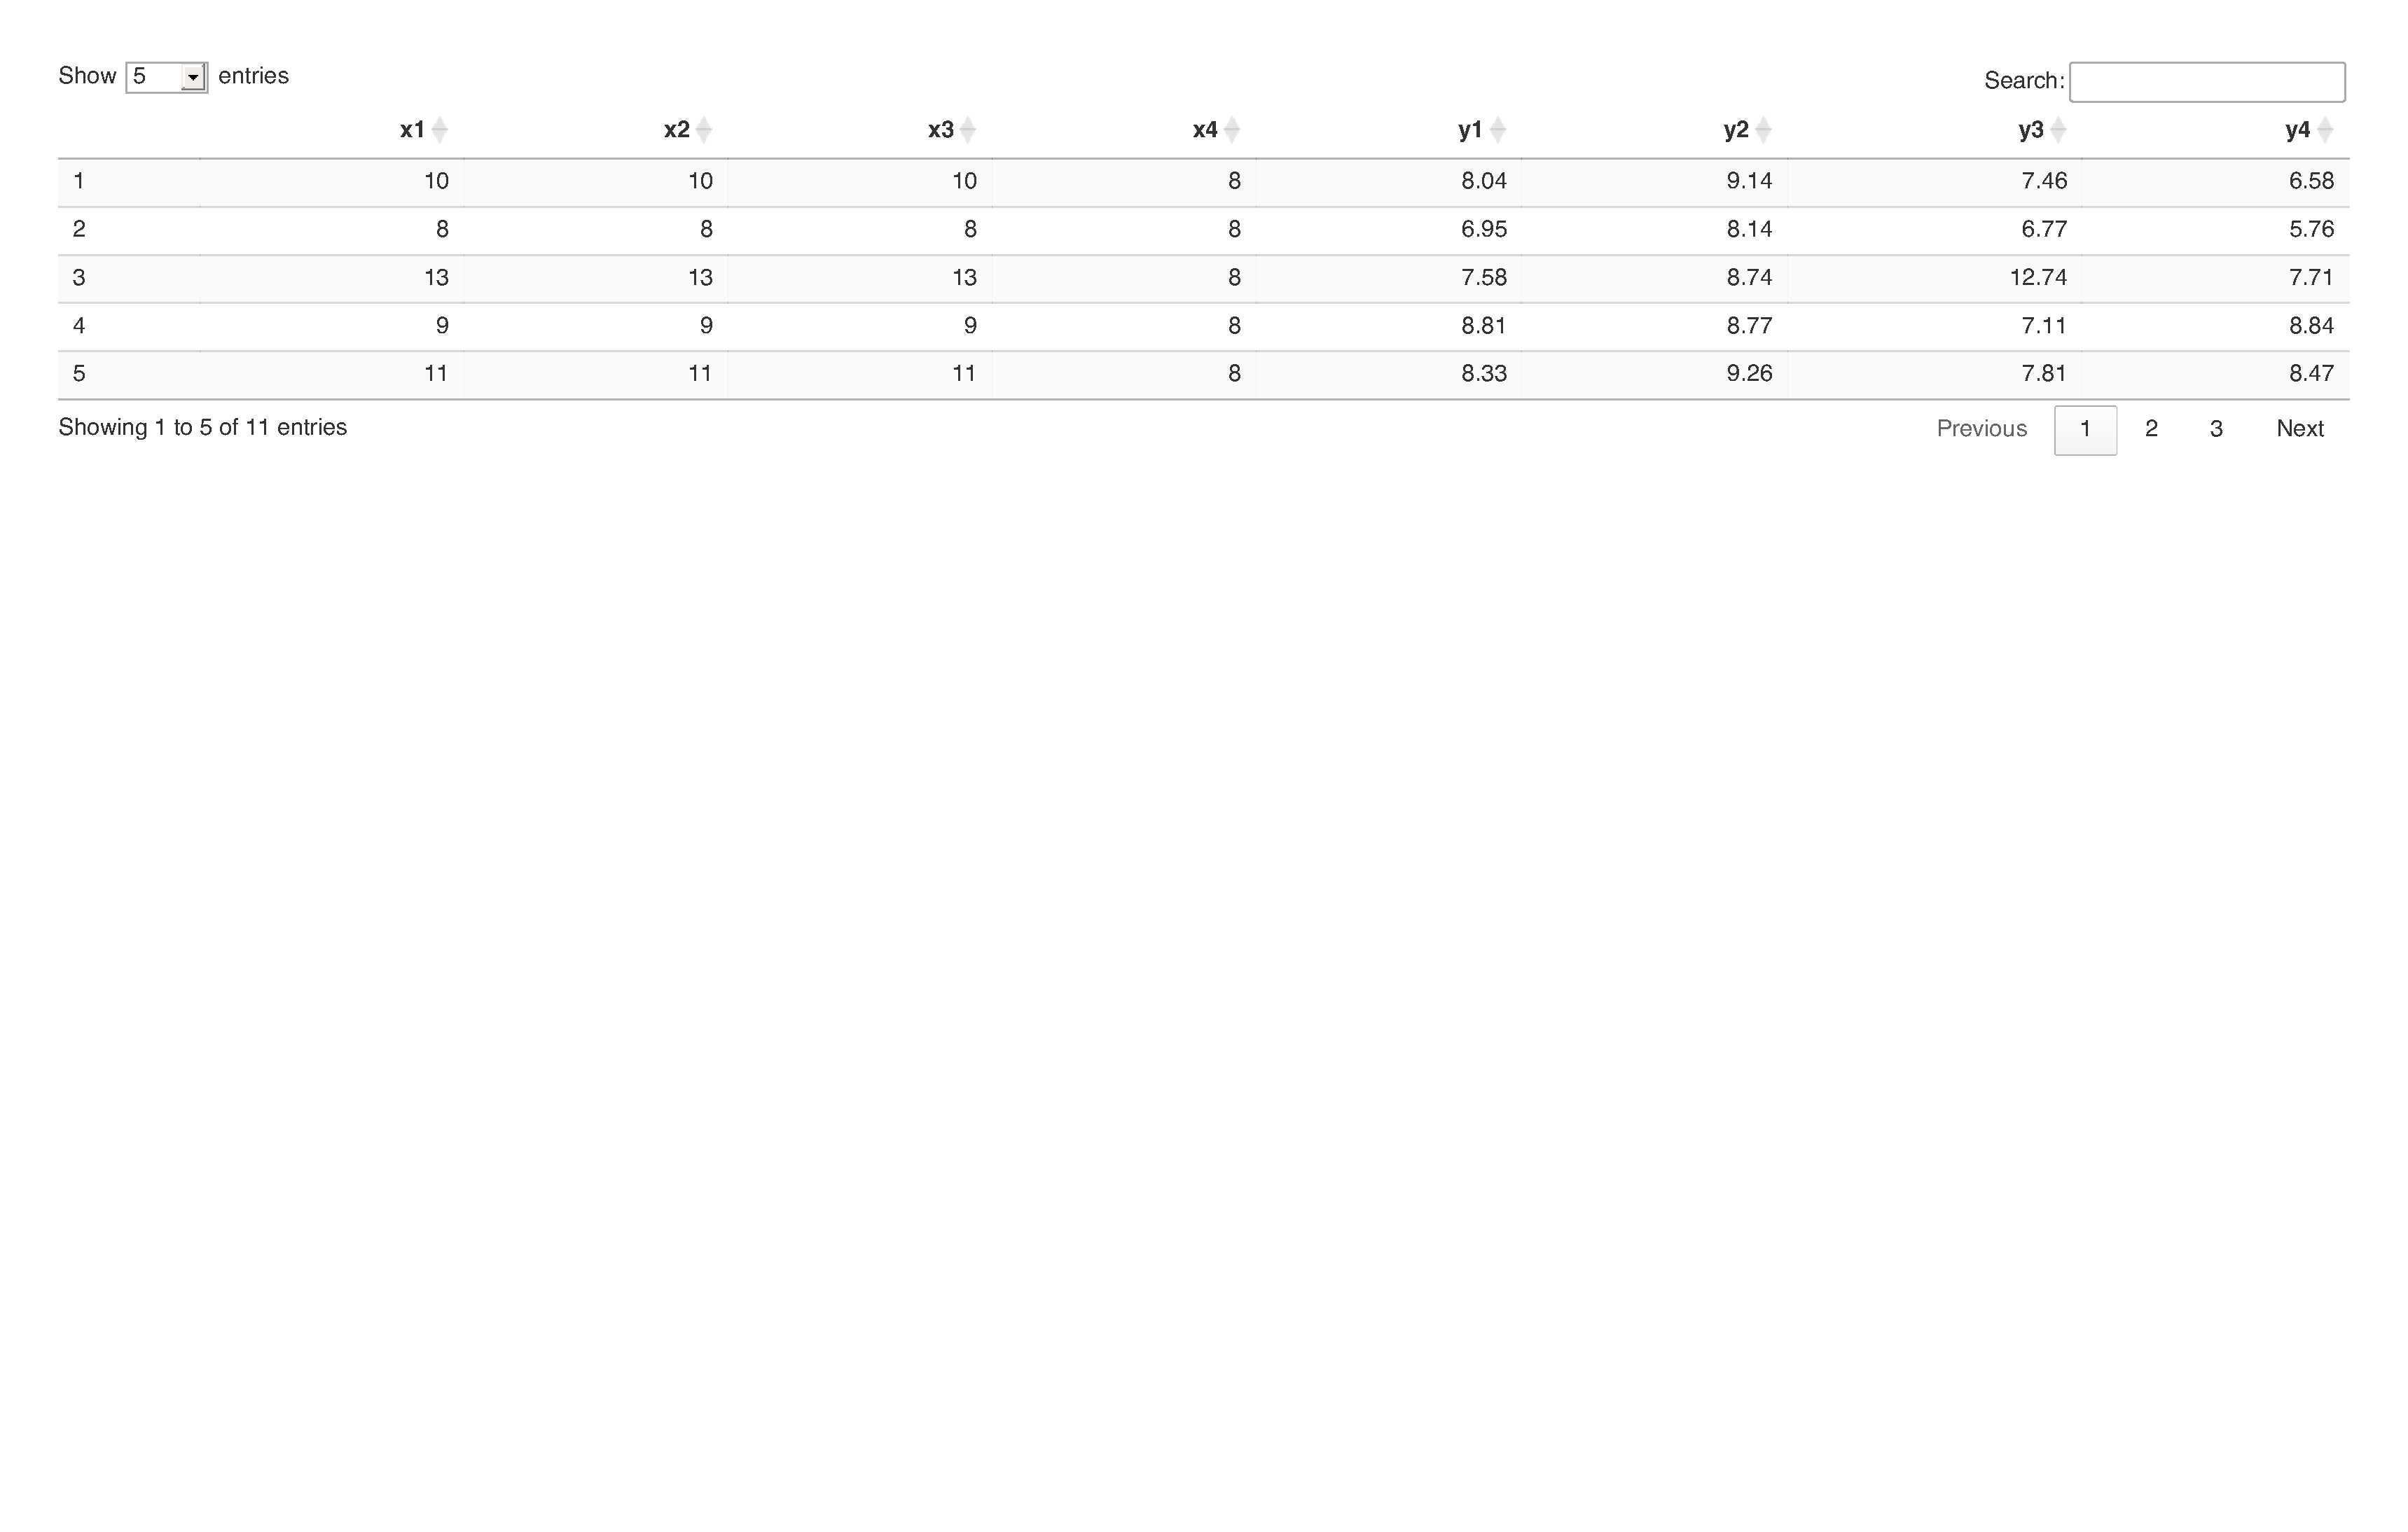
\includegraphics{voorbeelden_files/figure-pdf/tab-anscombe-1.pdf}

\part{Biologische modellering}

\usepackage{libertine}
\addtokomafont{disposition}{\rmfamily}
\renewcommand{\ttdefault}{clmt}

\providecommand{\ped}[1]{_\textrm{#1}}
\providecommand{\ap}[1]{^\textrm{#1}}
\providecommand{\app}[1]{^\textrm{#1}}

\providecommand*{\angs}{\smash{\mathrm{\ring A}}}
\providecommand*{\celsius}{\mathrm{~\circ C}}
\providecommand*{\micro}{\mu}

\providecommand*{\unit}[1]{\textrm{\,#1}}

\providecommand{\E}{\mathrm{e}}
\providecommand{\I}{\mathrm{i}}
\providecommand{\sfrac}[2]{^{#1}/_{#2}}

\providecommand{\conc}[1]{\left[\mathrm{#1}\right]}

\providecommand{\command}[1]{\textsl{#1}}
\providecommand{\out}[1]{\begin{verbatim}#1\end{verbatim}}

\providecommand{\diff}{\mathrm{d}\,}

\providecommand*{\deriv}[3][]{% arguments: order of the derivative(optional), function, variable
    \frac{\diff^{#1}#2}{\diff #3^{#1}}}
\providecommand*{\pderiv}[3][]{% arguments: order of the derivative(optional), function, variable
    \frac{\partial^{#1}#2}
        {\partial #3^{#1}}}

\renewcommand{\vec}[1]{{\boldsymbol #1}}

\providecommand{\cov}[2]{\mathrm{Cov}\!\left(#1, #2\right)}
\providecommand{\var}[1]{\mathrm{Var}\!\left(#1\right)}

\providecommand{\mean}[1]{\overline{#1}}

\providecommand{\sd}[1]{\sigma\left(#1\right)}
\providecommand{\ev}[1]{\mathbb{E}\!\left(#1\right)}
\providecommand{\pr}[1]{\textrm{Pr}\!\left(#1\right)}

\begin{figure}

\centering{


\includegraphics{Modellering/figuren/AI_models.jpeg}

}

\caption{\label{fig-AI_models}Modellering in de biologie, illustratie
gegenereerd door AI. (DALL-E 3, maart 2024)}

\end{figure}%

\chapter{Modellen in de biologie}\label{modellen-in-de-biologie}

\part{Statistiek voor biologen}

\begin{figure}

\centering{


\includegraphics{Statistiek/figuren/AI_statistics.jpeg}

}

\caption{\label{fig-AI_statistics}Statistiek voor biologien, illustratie
gegenereerd door AI. (DALL-E 3, maart 2024)}

\end{figure}%

\chapter{Wat is statistiek?}\label{wat-is-statistiek}

\section{bla}\label{bla}

\cleardoublepage
\phantomsection
\addcontentsline{toc}{part}{Bijlagen}
\appendix

\chapter{Eerse appendix}\label{eerse-appendix}




\end{document}
